% \documentclass[10pt,journal,compsoc]{IEEEtran}
% \usepackage{subfiles}
% \usepackage{url}
% \usepackage{amsmath}
% \usepackage{xspace}
% \usepackage{multirow}
% \usepackage{amssymb}
% \usepackage{algorithm}
% \usepackage{subfig}
% \usepackage[noend]{algpseudocode}
% \renewcommand{\algorithmicrequire}{\textbf{Input:~}}
% \renewcommand{\algorithmicensure}{\textbf{Output:~}}
% \newcommand\ovr[1]{\overrightarrow{#1}}
% \newcommand\myeq{\mkern1.5mu{=}\mkern1.5mu}
% \usepackage{booktabs}
% \usepackage{array}
% \usepackage{color}
% \usepackage{listings}
% \usepackage{placeins}
% \usepackage{enumitem}
% \usepackage{balance}
% \usepackage{etoolbox}
% \usepackage{lineno,hyperref}
% \newcommand\acrotwo{
% \multirow{2}{*}{ \shortstack{ \sc{Hyp.}\\\sc{Fus.}} }
% }
% \renewcommand{\toprule}{}
% \newcommand\acro{{\sc{HyperFuseR\xspace}\xspace}\xspace}
% \newcommand\kktodo[1]{\textcolor{red}{#1}}
% \newcommand\fixme[1]{\textcolor{red}{#1}}
% \newcommand\minspeedup{{{3.5\xspace}\xspace}\xspace}
% \newcommand\maxspeedup{{{11\xspace}\xspace}\xspace}
% \newcommand\maxspeedupTIM{{{1500\xspace}\xspace}\xspace}
% \newcommand\maxspeedupIMM{{{27.87\xspace}\xspace}\xspace}
% \newcommand\maxspeedupSKIM{{{11\xspace}\xspace}\xspace}

% \let\oldbibliography\thebibliography
% \renewcommand{\thebibliography}[1]{%
%   \oldbibliography{#1}%
%   \setlength{\itemsep}{0pt}%
% }

% \modulolinenumbers[5]

% \renewcommand{\floatpagefraction}{.98}
% % \journal{Journal of Parallel and Distributed Computing}

% %% `Elsevier LaTeX' style
% \bibliographystyle{elsarticle-num}
% %%%%%%%%%%%%%%%%%%%%%%%

% \begin{document}

% % \begin{frontmatter}
% % \title{Fast and Error-Adaptive Influence Maximization based on Count-Distinct Sketches}%\tnoteref{t1,t2}}

% % %% Group authors per affiliation:
% % %% or include affiliations in footnotes:
% % \author[add]{Gökhan Göktürk}
% % % \ead{gokhan.gokturk@sabanciuniv.edu}

% % \author[add]{Kamer Kaya}
% % % \ead{kaya@sabanciuniv.edu}

% % \address[add]{Faculty of Engineering and Natural Sciences, Sabancı University, Turkey}


% % \IEEEtitleabstractindextext{%
\documentclass[10pt,journal,compsoc]{IEEEtran}
\makeatletter
\long\def\@makecaption#1#2{\ifx\@captype\@IEEEtablestring%
\footnotesize\begin{center}{\normalfont\footnotesize #1}\\
{\normalfont\footnotesize\scshape #2}\end{center}%
\@IEEEtablecaptionsepspace
\else
\@IEEEfigurecaptionsepspace
\setbox\@tempboxa\hbox{\normalfont\footnotesize {#1.}~~ #2}%
\ifdim \wd\@tempboxa >\hsize%
\setbox\@tempboxa\hbox{\normalfont\footnotesize {#1.}~~ }%
\parbox[t]{\hsize}{\normalfont\footnotesize \noindent\unhbox\@tempboxa#2}%
\else
\hbox to\hsize{\normalfont\footnotesize\hfil\box\@tempboxa\hfil}\fi\fi}
\makeatother

%\DeclareUnicodeCharacter{2212}{-}
\usepackage[utf8]{inputenc}
\ifCLASSOPTIONcompsoc
  % The IEEE Computer Society needs nocompress option
  % requires cite.sty v4.0 or later (November 2003)
  \usepackage[nocompress]{cite}
\else
  % normal IEEE
  \usepackage{cite}
\fi

\newcommand\myeq{\mkern1.5mu{=}\mkern1.5mu}

\newcommand\MYhyperrefoptions{bookmarks=true,bookmarksnumbered=true, pdfpagemode={UseOutlines},plainpages=false,pdfpagelabels=true,
colorlinks=true,linkcolor={black},citecolor={black},urlcolor={black},
pdftitle={Fast and Error-Adaptive Influence Maximization based on Count-Distinct Sketches},%<!CHANGE!
pdfsubject={Typesetting},%<!CHANGE!
pdfauthor={G\"{o}khan G\"{o}kt\"{u}rk and Kamer Kaya},%<!CHANGE!
pdfkeywords={Influence Maximization, Graph Processing, Graph Sampling, Fused Sampling, Memory Access Regularization}}%<^!CHANGE!

\newcommand\rev[1]{{#1}}
% \newcommand\rev[1]{{#1}}
\usepackage{color,soul}
\definecolor{lightgray}{rgb}{0.83, 0.83, 0.83}
\DeclareRobustCommand{\hll}[1]{{\sethlcolor{lightgray}\hl{#1}}}
\newcommand\B[1]{\textbf{{{#1}}}}

\usepackage{amsfonts}
\usepackage{url}

\ifCLASSINFOpdf
  \usepackage[pdftex]{graphicx}
  \graphicspath{{./images/}}
  \DeclareGraphicsExtensions{.pdf,.jpeg,.png,.svg}
\else 
\fi
\usepackage{amsmath}
\usepackage{xspace}
\usepackage{multirow}
\usepackage{amssymb}
\usepackage{wrapfig}
\usepackage[]{booktabs}
\usepackage{algorithm}
\usepackage[noend]{algpseudocode}
\renewcommand{\algorithmicrequire}{\textbf{Input:~}}
\renewcommand{\algorithmicensure}{\textbf{Output:~}}
\newcommand\ovr[1]{\overrightarrow{#1}}
\newcommand\acro{{\sc{HyperFuseR\xspace}\xspace}\xspace}
\newcommand\kktodo[1]{\textcolor{red}{#1}}
\newcommand\ggx[1]{\textcolor{blue}{#1}}
\newcommand\fixme[1]{#1}
% \newcommand\fixme[1]{\textcolor{red}{#1}}
\newcommand\acrotwo{
\multirow{2}{*}{ \shortstack{ \sc{Hyp.}\\\sc{Fus.}} }
}
% \setlength{\intextsep}{1pt}%

\usepackage{array}
\usepackage{color}
\usepackage{listings}
\usepackage{placeins}
\usepackage{enumitem}
\newcommand{\resultsize}{0.6}
\algnewcommand{\algorithmicforeach}{\textbf{for each}}
\algdef{SE}[FOR]{ForEach}{EndForEach}[1]
  {\algorithmicforeach\ #1\ \algorithmicdo}% \ForEach{#1}
  {\algorithmicend\ \algorithmicforeach}% \EndForEach


\usepackage[caption=false,font=normalsize,labelfont=sf,textfont=sf]{subfig}

%\newcommand{\mycaption}[1]{\stepcounter{figure}\raisebox{-7pt}
%  {\footnotesize Fig. \thefigure.\hspace{3pt} #1}}



\begin{document}
\title{Fast and Error-Adaptive Influence Maximization based on Count-Distinct Sketches}
        

        
\author{G\"{o}khan~G\"{o}kt\"{u}rk
        and~Kamer~Kaya% <-this % stops a space
\IEEEcompsocitemizethanks{\IEEEcompsocthanksitem G. G\"{o}kt\"{u}rk and K. Kaya are with Computer Science and Engineering, Faculty of Engineering and Natural Sciences, Sabanci University, Istanbul, Turkey.}% <-this % stops a space
%\thanks{Manuscript received April 19, 2005; revised August 26, 2015.}}
}
%FIXME
\markboth{}%
{G\"{o}kt\"{u}rk \MakeLowercase{\textit{et al.}}: Boosting Parallel Influence-Maximization Kernels for Undirected Networks with Fusing and Vectorization}

\maketitle
\begin{abstract}
%     \fixme{
Influence maximization~(IM) is the problem of finding a seed vertex set that maximizes the expected number of vertices influenced under a given diffusion model. Due to the NP-Hardness of finding an optimal seed set, approximation algorithms are frequently used for IM. 
% }
In addition to these high-quality yet expensive approximation algorithms, lightweight, sketch-based approaches, which do not step-by-step simulate the diffusion process, have been proposed in the literature to cope with the scale of today's networks. 
In this work, we describe a fast, error-adaptive approach that leverages Count-Distinct sketches and hash-based fused sampling to estimate, not to count, the number of influenced vertices throughout a diffusion. We use per-vertex Flajolet-Martin sketches where each sketch corresponds to a sampled subgraph. To efficiently simulate the diffusions, the reach-set cardinalities of a single vertex are stored in memory in a consecutive fashion. This allows the proposed algorithm to estimate the number of influenced vertices in a single step for simulations at once. %In addition, thanks to their efficiency, and the scalability of our parallel implementation, we can rebuild the sketches whenever it is necessary. 
For a faster IM kernel, we rebuild the sketches in parallel only after observing estimation errors above a given threshold. Our experimental results show that the proposed algorithm yields comparable seed sets while being up to $3,337\times$ faster than a state-of-the-art, high-quality influence maximization algorithm. In addition, it is up to $63\times$ faster than a sketch-based approach while producing seed sets with $2\%$--$10\%$ better influence scores.
\end{abstract}
% } 
% \begin{keyword}
% Influence Maximization, Graph Processing, Graph Sampling, Fused Sampling, Memory Access Regularization, Count-Distinct Sketch
% \end{keyword}
% \end{frontmatter}


\section{Introduction}

Efficient information/influence dissemination in a network is an important research area with several applications in various fields, \fixme{such as viral marketing~\cite{leskovec2007dynamics, trusov2009effects}, social media analysis~\cite{zeng2010social, moreno2004dynamics}, and recommendation systems~\cite{lu2012recommender}.}
As the study of these networks is imperative for \fixme{educational, political, economic, and social purposes,} a high-quality seed set to initiate the diffusion may have vital importance.
Furthermore, since the diffusion analysis may be time-critical, or increasing the influence coverage may be too expensive, novel and efficient approaches to find good vertex sets that propagate the information effectively are essential.

Influence maximization is the problem of finding a subset $S \subset V$ of $K$ vertices in a graph $G = (V, E)$ with the vertex set $V$ and edge set $E$ such that $S$ reaches the maximum reachability, i.e., influences the maximum expected number of vertices, under some diffusion model. Kempe et al.~\cite{kempe2003maximizing} introduced the IM problem, \fixme{proved it to be NP-hard,} and provided a greedy Monte-Carlo approach that has a \fixme{constant approximation ratio over the optimal solution}. This greedy approach is one of the most frequently applied algorithms for IM. The time complexity of the greedy algorithm, with an influence score estimate $\sigma$, running $R$ simulations, and selecting $K$ seed vertices is $\mathcal{O}(KRn\sigma)$ for a graph with $n$ vertices. Although they perform well in terms of seed-set quality, the greedy Monte-Carlo solutions are impractical for real-life networks featuring millions of vertices as a consequence of their expensive simulation costs. Due to this reason, many \fixme{heuristics and proxy methods have been proposed in the literature~\cite{MixGreedy, narayanam2010shapley, kimura2007extracting, chen2010PMIA,chen2010LDAG, kim2013scalable, cohen2014sketch, goyal2011simpath, jung2012irie,cheng2014imrank,liu2014influence,galhotra2016holistic}}.

%%%%%%%%%%%%%%%%%%%%%%%%%%%%%%%%%%%%%%%%%%%%%%%%%%%%%%
%%%%%%%%%%%%%%%%%%%%%%%%%%%%%%%%%%%%%%%%%%%%%%%%%%%%%%
 
% However, these simulation-based, greedy algorithms provide the best possible approximation guarantees. Therefore they are considered as the gold standard for IM.  

Simulating a greedy algorithm in \fixme{parallel} is a \fixme{straightforward} workaround to reduce the execution time of IM kernels and make them scalable for large-scale networks. However, for large networks, a parallel, greedy approach with a good approximation guarantee does not come cheap on networks with billions of vertices and edges even if a large number of processing units/cores are available. Following similar attempts in the literature, we propose a parallel, sketch-based approach that approximates the Monte-Carlo processes. To boost the performance, the proposed approach does not exactly count the number of influenced vertices. Instead, it leverages Count-Distinct sketches. Below is a summary of our contributions:

\begin{itemize} [leftmargin=0.3cm]
\item \fixme{We propose \acro\footnote{\scriptsize{\url{https://github.com/ggokturk/infuser}}}, an open-source, blazing-fast, sketch-based and accurate Influence Maximization algorithm.} The proposed scheme samples the edges as they are traversed across several simulations. Thus, sampling, diffusion, and count-distinct processes are fused for all simulations. 

\item \fixme{Running concurrent simulations} on per-vertex Count-Distinct sketches reduces the number of memory accesses which is the main bottleneck for many graph kernels in the literature. While traversing an edge, \acro concurrently performs multiple diffusion simulations while using only a single (8-bit) value per vertex for each simulation. 

\item \acro{} can process large-scale graphs with millions of vertices and hundreds of millions of edges under a minute without compromising the quality of results. Furthermore, the performance scales near linearly with the number of threads available. In addition, while processing a large-scale graph, only a few GBs of memory is used, where most of the memory is spent for storing the graph itself. 

\item Once it is read from the memory, \acro processes all samples of a single edge together. The suggested approach, therefore, decreases the pressure on the memory subsystem. Furthermore, it employs vector compute units to its near maximum efficiency to regularize memory accesses.

\item We evaluate the runtime performance, memory consumption, and influence score of sketch- and approximation-based state-of-the-art influence maximization algorithms, namely {\sc Skim}~\cite{cohen2014sketch}, {\sc SSA}~\cite{nguyen2016stop}, {\sc Tim+}~\cite{tim} and {\sc Ripples}~\cite{minutoli2019fast}, to accurately position the performance of \acro{} within the IM literature. The experiments show that \acro can be $63\times$ and $3337\times$ faster than a state-of-the-art sketch-based and high-quality approximation algorithm, respectively while reaching the influence quality of the accurate algorithms with less memory.

\end{itemize}

% \fixme{The paper is organized as follows: 
% In Section~\ref{sec:background}, we present 
% the background on IM and introduce the mathematical notation. 
% Section~\ref{sec:method} describes the proposed approach in detail.}
% In Section~\ref{sec:evaluation}, a thorough performance evaluation \fixme{is provided by conducting experiments on various real-world datasets and influence settings. A detailed empirical comparison with the state-of-the-art from the literature is also given. Section~\ref{sec:relatedwork} presents a comparative overview of the existing work. Finally, Section~\ref{sec:conclusion} discusses future work and concludes the paper.}

%%%%%%%%%%%%%%%%%%%%%%%%%%%%%%%%%%%%%%%%%%%%%%%%%%%%%%
%%%%%%%%%%%%%%%%%%%%%%%%%%%%%%%%%%%%%%%%%%%%%%%%%%%%%%
\section{Notation and Background}\label{sec:background}

\fixme{Let $G = (V,E)$ be a} directed \fixme{graph where the $n$ vertices in $V$ represent the agents, and $m$ edges in $E$ represent the relations} among them. An edge $(u,v) \in E$ is an {\em incoming} edge for $v$ and an {\em outgoing} edge of $u$. The {\em incoming} \fixme{neighborhood of a vertex $v \in V$ is denoted as $\Gamma^-_{G}(v) = \{u: (u,v) \in E\}$.} Similarly, the {\em outgoing} neighborhood of a vertex $v \in V$ is denoted as $\Gamma^+_{G}(v) = \{u: (v,u) \in E\}$. A graph $G' = (V',E')$ is a sub-graph of $G$ if $V' \subseteq V$ and $E' \subseteq E$. The diffusion probability on the edge $(u, v) \in G$ is noted as $w_{u,v}$, where $w_{u,v}$ can be determined either by the diffusion model or according to the strength of $u$ and $v$'s relationship.

\begin{table}[!ht]
    \caption{Table of notations}
    \label{tab:notation}
          \renewcommand*{\arraystretch}{0.6}
    \centering
        \begin{small}
    % \tiny
    \begin{tabular}{|l|p{0.7\linewidth}|}
        \hline
        Variable & Definition  \\
        \hline
        %\kktodo{uzerinden 
        %gecelim}\ggx{A ekledim, S' uygun olur mu karar veremedim.}\\
        $G = (V,E)$     & Graph $G$ with vertices $V$ and edges $E$ \\
        $N$ & Number of vertices\\
        $M$ & Number of edges\\
        $T$ & Depth of the graph\\
        $\Gamma^+_G(u)$ & The set of vertices $v$ where $(u,v) \in E$ \\ %%FIXME
        $\Gamma^-_G(u)$  &The set of vertices $v$ where $(v, u) \in E$\\ %%FIXME
        $w_{u,v}$       & Probability of $u$ directly influencing $v$ \\
        %$SCC(v) $       & Strongly connected component of vertex $v$\\
        $R_{G}(v)$      & Reachability set of vertex $v$ on graph $G$\\
%        $\overline{R_{G}(v)} & Complement of the vertex set $R_{G}(v)$\\
        \hline\hline
        $S$             & Seed set to maximize influence\\
        $K$             & Size of the seed set\\
        ${\cal J}$   & Number of Monte-Carlo simulations performed\\
        $\sigma_{G}(S)$ & The influence score of $S$ in $G$, i.e., expected number of vertices reached from $S$ in $G$\\
        % $\sigma_{G}{(S,v)}$          & Marginal influence gain by adding vertex $v$ to seed set $S$\\
        \hline\hline
        $w_{u,v}$             & Sampling probability for the edge $(u,v)$\\
        $P(s,v)_r $     & Random probability generated for selecting edge vertices $s$ to $v$ in simulation $r$\\
        $h(u,v)$        & Hash function for edge $\{u,v\}$\\
        $h_{max}$       & Maximum value hash function $h$ can return\\
        %$X_r$           & Random number/hash generated for simulation $r$  \\
        \hline\hline
        $e$             & Estimated reachability set size\\
        % $[a, \ldots, a]_B$      & Vector of size $B$, contains all $a$\\
        $M_u[j]$        & $j$th sketch register for vertex $u$\\
        $\varsigma $    & Influence gained before last sketch build\\
        $\sigma $       & Influence Score\\
        $\delta$        & Marginal gain after last sketch build\\
        $err_l$         & Local estimation error of the sketch\\
        $err_g$         & Global estimation error of the sketch\\
        $\epsilon_{g}$    & Global estimation error threshold\\
        $\epsilon_{l}$    & Local estimation error threshold\\ 
        $\epsilon_{c}$    & Non-convergenced vertex threshold\\
      %  $x[[i, j]]$   & Slice of vector  $x$ between indices $i$ and $j$, not including $j$ \\ 
        \hline         
    \end{tabular}
    \end{small}
\end{table}
% \FloatBarrier
\subsection{Influence Maximization}

Influence Maximization aims to find a seed set $S \subseteq V$ among \fixme{all possible size $K$ subsets of $V$ that maximizes an {\em influence spread function} $\sigma$  when the diffusion process is initiated from $S$.} %Although we focus on graphs with bidirectional edges, for IM, the edges can be unidirectional depending on the initial construction. That is although the edges $\{u, v\} \in E$ are assumed to be bidirectional, throughout the diffusion process, we use $(u, v)$~($(v, u)$) as the edge that may be used to influence/activate $v$~($u$) given that $u$~($v$) has already been influenced/activated. This being said, $w_{u,v}$ can be set to zero to make the edge $(v, u)$ practically unidirectional. 
In the literature, {\em independent} and {\em weighted cascade}~(IC and WC), and 
{\em linear threshold}~(LT)~\cite{kempe2003maximizing} are three widely recognized diffusion models for IM. 

% \begin{figure}[!ht] 
%     \centering
%   \subfloat[\small{IC}\label{fig:ic}]{%
%        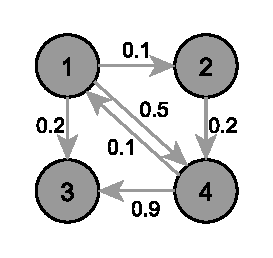
\includegraphics[width=0.4\linewidth]{images/ic.pdf}}
%   \subfloat[\small{WC}\label{fig:wc}]{%
%         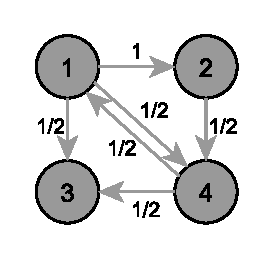
\includegraphics[width=0.4\linewidth]{images/wc.pdf}}
%     \\% IMAGES HERE
%   \caption{\small{\protect\subref{fig:ic} 
% The directed graph $G = (V, E)$ for IC with independent diffusion probabilities. 
% \protect\subref{fig:wc}
% The directed graph for WC is obtained by setting the diffusion probabilities of incoming edges to $1 / |\Gamma^-_G(v)|$ for each vertex $v \in V$.% \kktodo{bu (4,1) kenarinin agirligi 1 degil mi?}\ggx{done.} 
%   }}
%   %\label{fig_ic_model} 
%   \label{fig:xx} 
% \end{figure}

% \begin{itemize}[leftmargin=*]
% \item The {\bf Independent Cascade} model \fixme{works in rounds and activates} a vertex $v$ in the current round if one of $v$'s \fixme{incoming edges $(u, v)$ is used during the diffusion} round, \fixme{which happens with the activation probability $w_{u, v}$, given that $u$ has already been} influenced \fixme{in the previous rounds. The activation probabilities are independent (from each other and previous activations)} in the {\em independent cascade} model, which we focus on in this paper. A toy graph with activation probabilities on the edges is shown in Figure~\ref{fig:ic}.
% In theory, there can exist parallel and independent $\{u, v\}$ edges in $E$. In practice, they are merged to a single $\{u,v\}$ edge via preprocessing. 

% \item The {\bf Weighted Cascade}  model is a variant of the independent cascade that uses the structural properties of vertices to set the edge weights as shown in Figure~\ref{fig:wc}.
% The method, as described in~\cite{kempe2003maximizing}, sets $w_{u, v} = 1 / d_v$ where $d_v$ is the number 
% of incoming edges of $v$~(which in the original graph is equal to $\Gamma^-_G(v)$).
% Therefore, if $v$ has $\ell$ neighbors activated in the last round, its probability of activation in the new round is $1-( 1-1 / d_v)^\ell$. 
% %\kktodo{bu tanim [7]'dekine uymuyor. Orada undirected graph var }\ggx{fixed.} 
% % Note that the model is originally defined for undirected graphs in~\cite{kempe2003maximizing}. However, the definition above is consistent since one can consider each~(undirected) edge as two directed edges. 

% %$ {|E^G_{u,v}|}/{|E^G_{u}|}$ where $|E^G_{u,v}|$ is the number of parallel $\{u, v\}$ edges and $|E^G_{u}|$ is the number of $\{u, .\}$ edges, i.e., all of $u$'s edges in the undirected graph.

% \item{\bf Linear Threshold} model \fixme{generalizes} the IC \fixme{model and activates the vertex $v$} once the cumulative \fixme{activation coming} from its \fixme{neighbors} exceeds a given \fixme{threshold $\theta_v$}. 
% \fixme{All the $(u, v)$ edges with active $u$ vertices are taken into account} in the process. Vertex $v$ is activated when the total activation probability through these edges exceeds $\theta_v$~\cite{kempe2003maximizing}.  
% %Therefore, the independent cascade model is a special variant of the LT model with $\theta_v = 0$. 
% \end{itemize}

% \setlength{\columnsep}{1.2pt}%
\begin{wrapfigure}{r}{0.35\linewidth}
    \begin{center}
      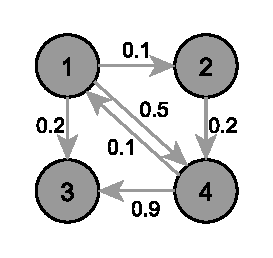
\includegraphics[width=1\linewidth]{images/ic.pdf}
    \end{center}
    \caption{\label{fig:ic}The directed graph $G = (V, E)$ for IC with independent diffusion probabilities.}
  \end{wrapfigure}
  The {\bf Independent Cascade} model \fixme{works in rounds and activates} a vertex $v$ in the current round if one of $v$'s \fixme{incoming edges $(u, v)$ is used during the diffusion} round, \fixme{which happens with the activation probability $w_{u, v}$, given that $u$ has already been} influenced \fixme{in the previous rounds. The activation probabilities are independent (from each other and previous activations)} in the {\em independent cascade} model, which we focus on in this paper. A toy graph with activation probabilities on the edges is shown in Figure~\ref{fig:ic}.
  % In theory, there can exist parallel and independent $\{u, v\}$ edges in $E$. In practice, they are merged to a single $\{u,v\}$ edge via preprocessing. 
%As a generalization of the above-mentioned models, {\bf triggering} has also been proposed by Kempe~et~al.~\cite{kempe2003maximizing}. In this model, each neighbor has a probability to influence the vertex $v$. The diffusion process chooses a random subset of vertices called the {\em triggering set} to activate the vertices at each instance.
The complexity analysis stays consistent for many diffusion models, including {\em Independent Cascade}, {\em Weighted Cascade}, and {\em Linear Threshold} models; the time complexity of the greedy algorithm, estimating the $\sigma$ influence score, running $R$ simulations, and selecting $K$ seed vertices is $\mathcal{O}(KRn\sigma)$ for a graph with $n$ vertices. 
We concentrate on the IC model in this paper, but although their adaptation requires some work, the proposed methods are also relevant to other models in the literature.

\subsection{Count-Distinct Sketches}\label{sec:sketch}

% \begin{figure}[!ht] 
%     \centering
%   \subfloat[\small{IC}\label{fig:fminit}]{%
%        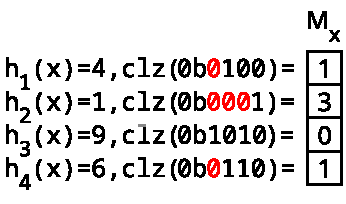
\includegraphics[width=0.5\linewidth]{images/fminit.pdf}}
%   \subfloat[\small{WC}\label{fig:fmmerge}]{%
%         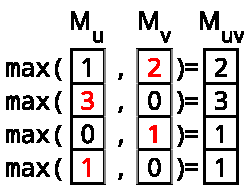
\includegraphics[width=0.5\linewidth]{images/fmmerge.pdf}}
%     \\% IMAGES HERE
%   \caption{\small{\protect\subref{fig:fm} 
% The directed graph $G = (V, E)$ for IC with independent diffusion probabilities. 
% \protect\subref{fig:wc}
% The directed graph for WC is obtained by setting the diffusion probabilities of incoming edges to $1 / |\Gamma^-_G(v)|$ for each vertex $v \in V$.% \kktodo{bu (4,1) kenarinin agirligi 1 degil mi?}\ggx{done.} 
%   }}
%   %\label{fig_ic_model} 
%   \label{fig:xx} 
% \end{figure}

The {\em distinct element count} problem focuses on finding the number of distinct elements in a stream where the elements are coming from a universal set ${\cal U}$. Finding the number of vertices to be influenced of a candidate seed vertex $u$, i.e., the cardinality of $u$'s {\em reachability set}, is a similar problem. For each sample subgraph, the number of visited vertices is found while traversing the subgraphs starting from $u$. Note that an exact, linear-time computation of stream cardinality requires memory proportional to the universal set cardinality, i.e., ${\Theta}(|{\cal U}|)$. Via sketches, \acro can estimate the reachability set cardinalities with much less memory and computation compared to the exact counting solutions. 

The reachability set of a vertex is the union of all its connected vertices (via outgoing edges). Many IM kernels exploit this property to some degree. The methods based on {\em reverse reachability} \cite{borgs2014maximizing} %\kktodo{cite}\ggx{done.} 
%and {\em bottom-up traversal} \\kktodo{cite} \ggx{buna referans dusunmem gerekli}
utilize this property directly to merge the reachability sets of connected vertices to estimate the number of vertices influenced. {\em MixGreedy} \cite{MixGreedy} %\kktodo{cite}\ggx{cited.} 
goes one step further; it utilizes the fact that for an undirected graph, all vertices in a connected component have the same reachability set. Therefore, all the reachability sets within a single sample subgraph can be found via a single graph traversal. 

For directed graphs, storing reachability sets for all vertices and merging these sets are infeasible for nontrivial graphs. 
If one-hot vectors are used to store the reachability sets for constant insertion time, $\Theta(n^2\mathcal{R})$ bits of memory are required where each merge operation has $\Theta(n)$ time complexity. 
If disjoints sets are used for storing reachability sets; $\mathcal{O}(n{\sigma}\mathcal{R})$ 
%\kktodo{Gokhan bunu aciklayalim, bir de $\bar{\sigma}$ nedir}\ggx{estimated influence} 
memory is required to store all reachability sets, and each merge operation has $\mathcal{O}({\tt Ack}(\sigma))$ complexity where ${\tt Ack}$ is the Ackermann~\cite{ackermann} function. %\kktodo{bu Ackermann'a atif verelim}.\ggx{done.}


Count-Distinct~Sketches can be leveraged to estimate a reachability set's cardinality efficiently; for instance, the Flajolet–Martin~(FM) sketch~\cite{flajolet1985probabilistic} uses a constant number, ${\cal J}$, of registers where ${\cal J}$ can be increased for better estimates. Furthermore, the union of two sketches can be computed in constant time which is a necessary property for an efficient estimation of reachability set cardinalities. The essence of an FM sketch is that it keeps track of how rare the elements are in a stream. The rarity of the stream is estimated by counting the maximum number of leading zeros in the stream elements' hash values. Initially, each register is initialized with zero. The items are hashed one by one, and the length of the longest all-zero prefix is stored in the register. With a single register, the cardinality estimation can be done by computing the power $2^r$ where $r$ is the value in the register.

In practice, multiple, ${\mathcal J}$, registers and hash values, $M[j]$ and $h_j$, $1 \leq j \leq {\cal J}$, are used to reduce the variance of the estimation. For a sketch with multiple registers, the impact of adding an item $x \in \cal{U}$ is shown in~\eqref{eq:sketch-add}:
\begin{equation}
    \label{eq:sketch-add}
    M[j] = \max(M[j], clz(h_j(x)),~1 \leq j \leq {\cal J}
\end{equation} where $clz(y)$ returns the number of leading zeros in $y$ and ${\cal J}$ is the number of sketch registers. With multiple registers, the average of the register values can be used to estimate the cardinality, and the result is divided to a correction factor $\phi \approx 0.77351$ to fix the error due to hash collisions. That is the estimated cardinality $e$ is computed as
\begin{equation}
    \label{eq:sketch-estimate}
    e = 2^{\bar{M}}/\phi
\end{equation} 
where $\bar{M} = {\tt{avg}}_j\{M[j]\}$ is the mean of the register values.

In this work, we utilize a variant of Flajolet–Martin sketch; since multiple Monte-Carlo simulations are performed to calculate the estimated influence, we use one register per simulation and take the average length of the longest leading zeros. Two given FM sketches $M_u$ and $M_v$ can be merged, i.e., their union $M_{uv}$ can be computed by taking the pairwise maximums of their registers. Formally; 
\begin{equation}
\label{eq:sketch-merge}
    M_{uv}[j] = \max(M_u[j], M_v[j]),~1 \leq j \leq {\cal J}.
\end{equation} 
In our implementation, the merge operations are performed if and only if there is a sampled edge between the vertices. %\kktodo{burada simulations yaziyordu, anlamadim, iki simulation arasinda nasil edge olur - o yuzden vertex yazdim}. \ggx{ j'th sampleda vertexler arasında sampled edge olmasını kastetmiştim. Yanlis olmus.}  


\section{Error-Adaptive Influence Maximization}\label{sec:method}

\acro{} uses {\em directed} fused sampling, utilizes \emph{sketches} for both influence estimation and seed selection, and a novel error-adaptive sketch rebuilding strategy. An IM tool leveraging fusing is~{\sc InFuseR}~\cite{infuser} which employs {\emph {undirected}} hash-based fused sampling and CELF optimizations~\cite{CELF} for seed selection to find the best seed set. Unlike {\sc InFuseR}, \acro{} follows a completely different approach and only estimates the cardinalities of the reachability sets and do not compute them. 

Most IM algorithms have the same few steps to find the best seed vertex set; sampling, building the influence oracle, verifying the impact of new candidates, and removing the latent seed set's residual reachability set. Following the idea proposed in~\cite{infuser}, \acro fuses the sampling step with other steps to avoid reading the graph multiple times. 

% \begin{wrapfigure}{l}{0.45\linewidth}
%     \begin{center}
%       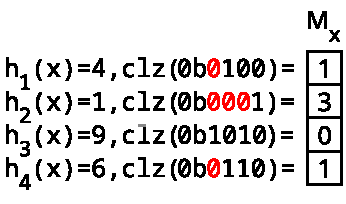
\includegraphics[width=1\linewidth]{images/fminit.pdf}
%     \end{center}
%     \caption{Toy sketch initialization of vertex $x$ with four registers and 4-bit hash functions.}
%   \end{wrapfigure}

% The method first performs a diffusion process; the process starts with per-vertex sketches that are initialized with the hash value of the corresponding vertex~(i.e., every vertex reaches to itself). Then, for all the (sampled) edges ($u, v$), i.e., for the ones that contribute to the diffusion for this simulation, the sketch of the source vertex $u$ is merged into that of the target vertex $v$ until all sketch registers for all the vertices converge. The merge operation utilized in this process is slightly different from the conventional one and retrofitted to mimic the IC diffusion. 

% \begin{wrapfigure}{l}{0.35\linewidth}
%     \begin{center}
%       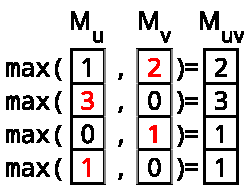
\includegraphics[width=1\linewidth]{images/fmmerge.pdf}
%     \end{center}
%     \caption{\label{fmmerge} Example of union operation on sketches of vertices $x$ and $y$ with four registers.}
%   \end{wrapfigure}


%At each iteration, the sketches of the existing reachable vertices are modified. \kktodo{onceki cumleyi de degistirdim - dogru mu} \ggx{her vertex başkasına reachable olabilir, son cumleyi çıkartabilirz}
%Instead of simulating the diffusion sample-by-sample, vertex-by-vertex, or path-by-path, all the influence that passes through the edges in a single step is processed together. 

% \begin{wrapfigure}{l}{0.35\linewidth}
%     \begin{center}
%       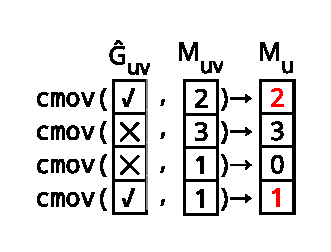
\includegraphics[width=1\linewidth]{images/fmwrite.pdf}
%     \end{center}
%     \caption{Example of writing merged sketch $M_{xy}$ in fig.\ref{fmmerge} back to $M_x$ w.r.t diffusion process.}
%   \end{wrapfigure}

\acro performs $K$ iterations to find $K$ vertices. Each iteration starts by estimating the reachability set cardinalities for all the vertices and keeping this information within sketches. After this, \acro picks the vertex $v$ with the largest cardinality by evaluating these sketches. It then finds the (actual) reachability set of the latent seed set, which is the union of the reachability sets of $v$ and the vertices in the seed set, by performing Monte-Carlo simulations. The vertices in this reachability set are removed from the live set $L$. %labeled as {\em visited}. 
%\kktodo{niye blocked, influenced desek?}\ggx{literaturde kullanilan terim o sekilde, ben visited'i tercih ederdim, algorithmaya gore live set L den çıkartıyoruz diye güncelledim.} 
Hence, in later iterations, these vertices will not contribute to the marginal gain. Although the same sketch memory can be used for a couple of iterations, i.e., seed vertex searches, we have observed that sketches become dirty and a rebuild is necessary. Hence, finally, the algorithm checks if sketch rebuilding is necessary based on the difference between the sketch estimate and Monte-Carlo estimate. The proposed approach and the algorithm is described here in more detail starting with fused sampling.%\kktodo{yukaridaki cumlelerde bunlara isim verelim, burada soyleyelim matematiksel olarak - zaten isimleri var sanirim}.\ggx{malesef sembolleri,isimleri yok. $u \notin R_S$ şeklinde.} 

\subsection{Hash-based Fused Sampling}
The probabilistic nature of cascade models \fixme{requires} sampling \fixme{subgraphs from $G = (V, E)$ to simulate the diffusion process}. If performed individually as a preprocessing step, as the literature traditionally does, sampling can be an expensive stage, furthermore, a time-wise dominating one for the overall IM kernel. That is first, sampling multiple sub-graphs may demand multiple passes on the graph, which can be very large and expensive to stream to the computational cores, and second, if samples are memoized, the memory requirement can be a multiple of the graph size. 
In this work, we borrow the fused-sampling technique from {\sc InFuseR}~\cite{infuser} which eliminates the necessity of creation and storage of the sample subgraphs in memory. 
In Fig.~\ref{fig:traversal}, we illustrate fused-sampling; instead of processing the samples independently as in Fig.~\ref{fig:sims}, fused-sampling processes each edge concurrently for multiple simulations as shown in Fig.~\ref{fig:fused}. This allows us to process each edge only a few times instead of once per simulation.


\begin{figure}[!ht] 
    \centering
    %\subfloat[\label{fig:toy}]{%
    %   \includegraphics[width=0.47\linewidth]{sims-a%}}%  \\
    \subfloat[\label{fig:sims}]{%
        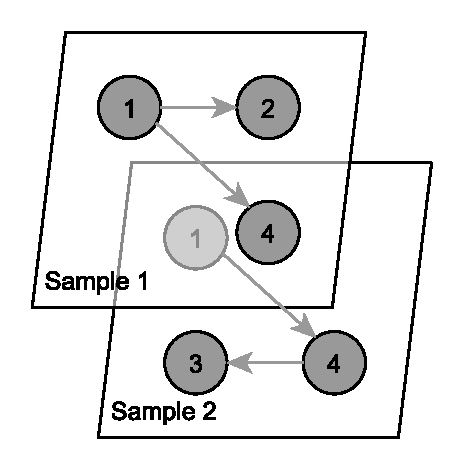
\includegraphics[width=0.5\linewidth]{images/samples.pdf}
    } 
    \subfloat[\label{fig:fused}]{%
     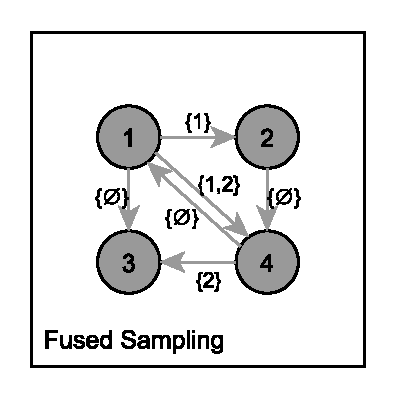
\includegraphics[width=0.5\linewidth]{images/fused.pdf}}
  \caption{\small{
  %\protect\subref{fig:toy} The toy graph 
  \protect\subref{fig:sims} Two sampled subgraphs of the toy graph from Figure~\ref{fig:ic} with 4 vertices and 6 edges.
  \protect\subref{fig:fused} The simulations performed are fused with sampling. Each edge is labeled with the corresponding sample/simulation IDs. 
  }}
  \label{fig:traversal} 
\end{figure}

In \acro, when an edge of the original graph is being processed, it is processed for all possible samples. Then, it is decided to be {\it sampled} or {\it skipped} depending on the outcome of the hash-based random value for each sample. Given a graph $G = (V, E)$, for an edge $(u, v) \in E$, the hash function used is given below:
% \begin{equation}
%     \label{eq:hash}
%     h(u,v) = \mbox{{\sc CRC32}}(u||v)~mod~2^{31}  
% \end{equation} %FIXME: does this mean this value be negative?

\begin{equation}
    \label{eq:hash}
    h(u,v) = \mbox{{\sc Hash}}(u||v)~mod~2^{31}  
\end{equation} %FIXME: does this mean this value be negative?
where $||$ is the concatenation operator. 
% In our preliminary experiments, we have tried a set of hash algorithms and found that {\sc Crc32}~\cite{koopman200232} and {{\sc Murmur3}} are good candidates for {\sc Hash}. {{\sc Murmur3}} was slightly faster than {\sc Crc32} with better randomness properties. 
% After a preliminary analysis, \fixme{we chose {{\sc Murmur3}} due to its simplicity and good avalanche behavior with a maximum bias $0.5\%$~\cite{MurmurHash3Performance}.} 
An  important bottleneck of hash-based fused sampling is the need of the hash value for an edge whenever it is read from the memory. To mitigate its overhead, using $\Theta(|E|)$ more memory, we precompute and memoize the hash values (and read them when we need them). We have also tried recomputing the hash values every time they are needed; this incurred around $5\%$ slowdown. Since {\acro} is designed for multi-core servers, extra $\Theta(|E|)$ memory is a practical overhead. However, considering its low overhead, the recomputation strategy can be promising for memory-restricted accelerators and devices such as GPUs.

% Although the $h(.)$ function described above \fixme{generates a unique hash value for each edge, and hence can be used to generate a unique sampling probability, different simulations require different probabilities.} To enable this, 

A set of uniformly \fixme{ randomly chosen numbers $X_r \in_R [0, h_{max}]$ } associated with each sample $r$ are generated for each edge to generate a unique sampling probabilities for all samples. Then, the sampling probability of $(u, v)$ for simulation $r$, $P(u, v)_r$, is computed: the hash value, $h(u,v)$, is XOR'ed with  $X_r$ and the result is normalized by dividing the value to the upper limit of the hash value $h_{max}$. Formally,
\begin{equation}
    \label{eq:hash_prob}
    P(u,v)_r = \frac{X_r \oplus h(u,v)}{h_{max}}.
\end{equation}
% The edge $\{u,v\}$ is verified to be in the sample if ${\rho}(u,v)_r$ is smaller than or equal to the threshold $w_{u,v}$. 
The edge $(u,v)$ exists \fixme{in the sample $r$ if and only if  ${P}(u,v)_r$ is smaller than the edge threshold $w_{u,v}$.} One of this approach's benefits is that an edge can be sampled using \fixme{a single XOR and compare-greater-than operation} which is crucial since \acro{} recomputes this probability value each time the corresponding edge is read from the memory. In practice, we do not apply the division operation since $h_{max}$ is a constant value and the same for every edge and simulation. Moreover, the corresponding control flow branch overhead can be \fixme{removed} using {\em conditional move} \fixme{instructions}. 

% \begin{figure}[!ht] 
%     \centering
%     \includegraphics[width=0.8\linewidth]{./images/CDF.pdf}
%     \caption{\small{Cumulative probability function of hash-based sampling probabilities on various real-life networks.}}
%     \label{fig:prob-cdf} 
% \end{figure}

% Using a strong hash function such as {{\sc Murmur3}} ensures that all bits independently change if the input is changed. This property allows us to generate good-enough pseudo-random values for fair sampling. To evaluate the randomness and fairness of the values generated with the hash-based approach, we generated a large number of samples for various real-life networks and plotted the cumulative distribution.
% and the bias of the random values $P(u,v)_r$ used~(Fig.~\ref{fig:prob-bias}). 
% As Figure~\ref{fig:prob-cdf} shows, the sampling distribution of the hash-based computation values resembles a uniform random distribution. 
% Furthermore, the latter shows that the bias is insignificant for each network. 

% \begin{figure}[!ht] 
%     \centering
%     \includegraphics[width=1\linewidth]{./images/bias.pdf}
%     \caption{\small{Bias distribution of hash-based sampling probabilities on various real-life networks.}}
%     \label{fig:prob-bias} 
% \end{figure}

% For a given graph $G = (V,E)$, the bias of a sampling probability $x$ is computed as $|(31/2) − E(|H(m)|) / E(|H(m)|))|$ for all $(u,v) \in E$ and $0 \leq r < R$. 
% Figure~\ref{fig:prob-bias} shows the bias for 12 real-life networks. 
%Traditional implementations sample each edge in $G$ once per simulation and store them to construct a sampled subgraph. n
%Being able to generate the samples on the fly allows us to avoid many memory accesses. 
% One of the downsides of hash-based fused sampling is that we have to generate all these random values,  $P(u,v)_r$, for each edge traversal and each simulation $r$. As mentioned above, the edges' hash values are precomputed for all the edges in $E$ to reduce computation cost and leverage fused sampling's performance gains. %Fortunately, the rest of the operations, i.e., one XOR and one division, are very fast on modern computing hardware. %The trade-off between extra memory and computation here maybe not be applicable for different computation architectures and faster/simpler hash functions.
\subsection{Estimating Reachability Set Cardinalities}

To estimate the cardinality of a reachability set, \acro{} performs a cheap diffusion process over the sample subgraphs by using a single sketch register for a single sample/simulation. 
For an edge ($u, v$) in simulation $j$ where $v$ is a live vertex, an update, i.e., a merge operation, on $u$'s register is performed on the corresponding register $M_u$[$j$], i.e., $M_u[j] = max(M_u[j],M_v[j])$. 
The toy example in Fig.~\ref{fig:fmops} with  ${\cal J} = 4$ shows how the sketch operations are done on a toy problem. In Fig.~\ref{fig:fmops}(a), the sketches, in a toy problem with 4 samples and 4-bit hash functions, are initialized; the id of vertex $u$ is hashed and leading zeros of the hash are written to registers. In Fig.~\ref{fig:fmops}(b), the merge operation is illustrated on registers of vertex $u$, $M_u$, and vertex $v$, $M_v$; merge operation takes element-wise maximum of registers to find union of the reachability sets. All these operations are performed using vectorized instructions. 

 To vectorize the rest of the process, we leverage conditional move operations. Although an edge ($u, v$) is inside the graph, it may not be in all the samples. In the toy example of Fig.~\ref{fig:fmops}, we assume that ($u, v$) only exists in the first and the last sample. 
 Fig.~\ref{fig:fmops}(c) writes the merged reachability sets back to $u$'s registers. For the first sample, $M_u[1]$ needs an update. The operations for the second and the third rows/samples are skipped since ($u, v$) does not exist in these samples. The fourth row shows the case with ($u$, $v$) is in the sample but $M_u[4] < M_v[4]$. Hence, the move operation is not needed. However, for such cases, we still perform this write as a part of the vectorized operation. This being said, we skip the whole Fig.~\ref{fig:fmops}(c) when ($u, v$) is not in any of these samples.   

%if and only if the edge exists in the sample and \kktodo{bunu da degistirdim}\ggx{biz bunu yapmiyoruz, ben burada kayboldum.} $u$ is {\em live} in the current iteration. 
%A merge operation between sketch $M_u$,$M_v$ of vertices $u$,$v$,is only performed on $j$th register if there is a live edge between $u,v$ in sample $j$.

\begin{figure}[!ht]
    \begin{center}
    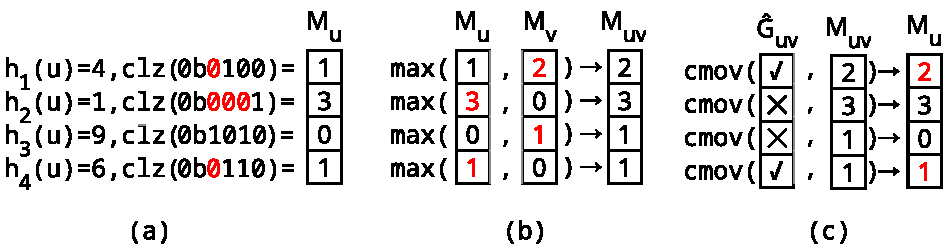
\includegraphics[width=\linewidth]{images/fmops.pdf}
    \caption{ (a) \label{fminit} Toy sketch initialization of vertex $u$ with four registers and 4-bit hash functions. (b) \label{fmmerge} Example of union operation on sketches of vertices $u$ and $v$ with four registers. (c) \label{fmwrite} Diffusion operation from vertex $v$ to vertex $u$ w.r.t. sampled subgraph. 
     }\label{fig:fmops} 
    \end{center}
\end{figure}

To summarize, at each iteration, vertices (outgoing) neighbors' reachability sets are added to their sketches.
This recursive formulation of the influence iteratively relays the reachability information among the vertices, allowing us to estimate the marginal influence for all vertices very fast.

\subsection{Finding the Seed Set}
A greedy solution to IM requires finding a vertex with a maximum marginal influence at each step until the seed set size reaches $K$.
An exact computation of marginal influences, i.e., the additional influence when a vertex $v$ is added to the seed set, requires the computation of all candidate vertices' reachability sets within all the samples. This involves many graph traversals and is expensive even with various algorithmic optimizations and a scalable parallelized implementation, e.g., see~\cite{infuser}. %The influence estimation problem is quite similar to the Count-Distinct problem applied to all sample subgraphs, as explained above. Hence, 
In this work, we pursue the idea of using Count-Distinct sketches to estimate marginal influence scores. Here we propose an efficient and effective IM algorithm, \acro, that utilizes Flajolet–Martin sketches described in Section~\ref{sec:sketch} to estimate the averages of distinct elements in the sampled subgraphs. Algorithm~\ref{algo:main} shows the steps taken by \acro.

\renewcommand{\baselinestretch}{0.95}
\begin{algorithm}
\caption{\sc{\acro}($G,K,{\cal J}$)}
\label{algo:main}
\algorithmicrequire{$G = (V,E)$: the influence graph
\\\hspace*{6.6ex}{$K$: number of seed vertices
\\\hspace*{6.7ex}${\cal J}$: number of Monte-Carlo simulations}\\}
\algorithmicensure{$S$: a seed set that maximizes the influence on $G$
}
\begin{algorithmic}[1]
    \State {$S \leftarrow \{\emptyset\}$}
    \For{$ v\in V$} {\bf in parallel}
        \For{$ j \in \{1, \ldots, {\cal J}\}$}
            \State $M_v[j] \leftarrow clz(hash(v) \oplus hash(j))$ 
        \EndFor
    \EndFor
    \State $M \leftarrow ${\sc Simulate}$(G,M,{\cal J},\emptyset)$
    \State $M_{S'} \leftarrow zeros({\cal J})$
    \State $\varsigma \leftarrow 0$
    \For{$k=1\ldots K$} \label{line:for}
        \State $s \leftarrow \underset{v\in V}{\mathrm{argmax}}\{${\sc Estimate}$(${\sc Merge}$(M_{S'},M_v))$\}\label{line:estimate}
        
        %\kktodo{S' nedir}\ggx{ latent seed set after rebuild}
        \State $S \leftarrow S \cup \{s\}$     
        \State $e \leftarrow ${\sc Estimate}$(${\sc Merge}$(M_{S'},M_s))$\label{line:e}
        % \State $R_S \leftarrow run\_cascade(G,S,{\cal J})$
        %\State {Compute $R_{G}(S)$; the reachability set of $S$}
        %\kktodo{buna da bir algoritma eklesek} }\ggx{Yayın konusu dışında kalabilir diye çıkartmıştık.}
        \State $R_G(S) \leftarrow$ reachability set of $S$ (for all simulations)
        \State $\sigma \leftarrow$ Monte-Carlo-based (actual) influence of $S$
        \State $\delta = \sigma - \varsigma$
        \State $err_l=|(e - \delta) / \delta|$
        \State $err_g=|(e-\delta) / \sigma|$
        \If{$ err_l < \epsilon_l \lor err_g < \epsilon_g$} %FIXME
            \State $M_{S'} \leftarrow$ {\sc Merge}$(M_{S'},M_s)$ \label{line:if}
        \Else 
            \For{$ v\in V$} {\bf in parallel}\label{line:else1}
                \For{$ j \in \{1, \ldots, {\cal J}\}$}
                    \State $M_v[j] \leftarrow clz(hash(v) \oplus hash(j))$ 
                \EndFor
            \EndFor
            \State $M \leftarrow ${\sc Simulate}$(G,M,{\cal J},R_{G}(S))$
            \State $M_{S'} \leftarrow zeros({\cal J}) $ 
            \State $\varsigma \leftarrow \sigma $ \label{line:else2} 
        \EndIf
    \EndFor
    \State \Return $S$
\end{algorithmic}
\end{algorithm}
\renewcommand{\baselinestretch}{1}

 Algorithm~\ref{algo:main} first initializes the reachability sets of all vertices by adding the vertices themselves. 
 That is for all vertices $u$, its $j$th register is set to $M_u[j]=clz(h_j(u))$ meaning $R_{{G}_j}(u) = \{u\}$ where $G_j$ is the $j$th sampled graph. 
 Then, we perform the diffusion process on the sketch registers whose pseudocode is given in Algorithm~\ref{algo:diffusion-step}. The diffusion starts by adding all the vertices to the {\em live vertex set} $L$. 
 Then at each step, the incoming edges of the live vertices are processed. 
 For a vertex $u$, its sketch, $M_u$, is updated by merging the sketches $M_v$ of all live outgoing neighbors vertices $v \in {L} \cap \Gamma^+_{G}(u)$. For each such vertex $v$ and simulation $j$, the operation $M_u[j] = max(M_u[j], M_v[j])$ is performed. This approach can be seen as a bottom-up, i.e., reversed,  diffusion process where at each iteration, the cardinality information is pulled from vertices neighbors.


%  If a vertex $u$ is live, its outgoing edges $(u, v)$ s.t. $v \in \Gamma_G(v)$ are processed and the sketches of $v$ are merged into those of $u$. \kktodo{burada edgeleri tersten process ettigimizi aciklamamiz gerek} burasi yanlis
If any of $u$'s sketch registers changes during this operation, it is added to the live vertex set $L'$ of the next iteration. Once the incoming edges of all live vertices are processed, the iteration ends. 
% Figure~\ref{fig:hf-processing} shows how \acro performs two simulations at the same time using sketch registers.
 
 
\renewcommand{\baselinestretch}{0.95}
\begin{algorithm}[!ht]
\caption{\sc{Simulate}($G,M,{\cal J},R_S$)}
\label{algo:diffusion-step}
\algorithmicrequire{$G = (V,E)$: the influence graph
\\\hspace*{6.6ex}{$M$: sketch vectors of vertices
\\\hspace*{6.7ex}${{\cal J}}$: number of MC simulations
\\\hspace*{6.7ex}$R_S$: reachability set of the seed set
}
\\}
\algorithmicensure{$M$: updated Sketch vectors
}
\begin{algorithmic}[1]
    \State {$L \leftarrow V$}
    \State {$L' \leftarrow {\emptyset}$}
    \While{$|L|/|V| > \epsilon_c$}
        \For{$u \in \Gamma(L)$} {\bf in parallel} \label{ln:inner_start} %REVERSE THIS
        \For{$e_{u,v} \in A(u) $}
            \For{$j \in (0,{\cal J}]$} \label{ln:vec1}
                \If{$P(u,v)_j < w_{u,v} \land u  \not\in R_S[j]$} \label{ln:early_exit}
                    \State{$M_u[j]\leftarrow max(M_u[j],M_v[j])$}\label{ln:update}          
                \EndIf
            \EndFor
            \If {$M_u$ changed}
                \State $L' \leftarrow L' \cup u $ \label{ln:inner_end}
            \EndIf
        \EndFor
        \EndFor
        \State $L \leftarrow L'$
        \State $L' \leftarrow \{\emptyset\}$
    \EndWhile
    \State \Return $M$
\end{algorithmic}
\end{algorithm}
\renewcommand{\baselinestretch}{1}

 
% \begin{figure*}[!ht]
%     \begin{center}
%     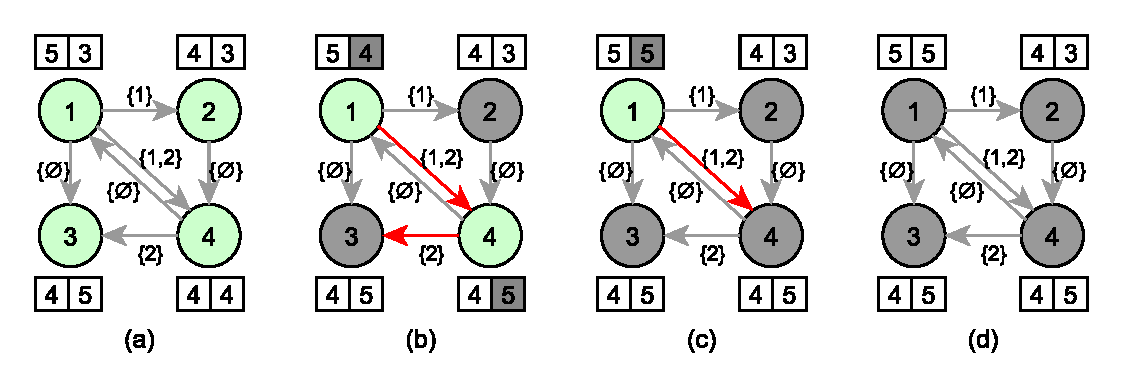
\includegraphics[width=0.85\linewidth]{images/sketch-diffusion.pdf}
%     \caption{\small{(a) The initial state on the toy graph for \acro{}; all vertices are set as live~(green), and their registers are initialized with the length of the zero prefix of their hashes. (b) 
%     % For all live edges,$e_{ij}$, respective registers are merged and set to source vertex $j$'s register, $M_j \leftarrow Max(M_i, M_j)$. 
%     For the ($1, 4$) edge which is live for both simulations, 1's registers are set to the maximum of both 1's and 4's registers. The ($4, 3$) edge is live only in the second simulation. Hence, the second register of $4$ is updated to $5$. For the second iteration, vertices 1 and 4 are live~(green) since their registers have changed. (c) For the live ($1, 4$) edge, 1's second is updated and 1 is set as live again. (d) All the registers converged. As no live vertices exist, the process stops.}}\label{fig:hf-processing} 
%     \end{center}
%     \end{figure*} 
 
The traditional Greedy algorithm~\cite{kempe2003maximizing} processes the simulations one-by-one and computes the vertices' reachability sets. On the other hand, \acro efficiently performs multiple simulations at once in a single-step iteration (which processes distance-1 neighborhoods). Since each iteration relays one level of cardinality information, this step requires at most $d$ iterations where $d$ is the diameter of $G$. Note that when processed individually (as the Greedy algorithm), the $j$th simulation over the sampled subgraph $G_j$ would require only at most $d_j$ iterations, which is the diameter of $G_j$, and probably much smaller than $d$ considering the sampled subgraphs being highly sparse. However, $d$ is also a loose upper bound for \acro. A better one is {\tt max}$\{d_j: 1 \leq j \leq {\cal J}\} + 1$ where $d_j$ is the diameter of $G_j$. We have observed that during these simulations later iterations have only a minor impact on the marginal influence scores. Hence, to further reduce the overhead of concurrent simulation processing and avoid bottleneck simulations due to remaining perimeter structures (e.g., paths on the perimeter), we employ an early-exit threshold $\epsilon_c$ over the remaining live vertices ratio, which is expected to be very small when only one or two (bottleneck) simulations remain. That is if $|L'| \leq |V| \times \epsilon_c$ the diffusion process in Algorithm~\ref{algo:diffusion-step} stops. Otherwise, $L$ is set to $L'$, $L'$ is cleared, and the next iteration starts. We used $\epsilon_c = 0.02$ to make \acro faster while keeping its quality almost the same. 

Figure~\ref{fig:hyperdiff} shows a toy diffusion process on four vertices and a single sample. The process initializes sketches using respective hashes' number of leading zeros. Then larger numbers are started to be pulled from all recently changed neighbors. The same process is repeated for multiple vertices until the new seed vertex is found. To understand the benefits of estimating (instead of counting), we present Fig.~\ref{fig:infuserdiff} which shows an example in the same settings as Fig.~\ref{fig:hyperdiff}. One very important observation is that, in these examples, \acro{} computes the estimated influence for \emph{all} vertices with a single process, whereas {\sc InFuseR}, or another counting-based IM algorithm, only computes influence for a single vertex (vertex one in the example). Doing otherwise, i.e., computing the reachability set cardinalities for all the vertices at once for a given sample, may require $\mathcal{O}(n^2)$ memory and union operations with $\mathcal{O}(n)$ complexity. Although using CELF~\cite{CELF} optimization partially eliminates this problem by focusing only a few vertices, $\mathcal{O}(n)$ union complexity still remains.
%This is why although the reachability sets in Fig.~\ref{fig:infuserdiff} are shown for all vertices with dense vectors, the ones except that of vertex 1 are greyed out since they are not manipulated.
\begin{figure}[!ht]
    \begin{center}
    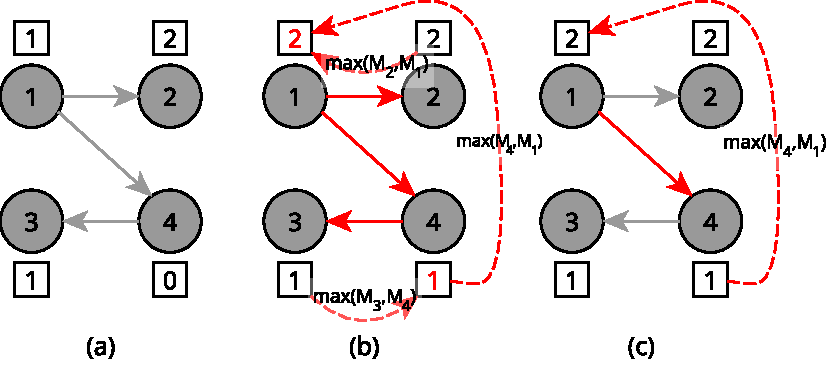
\includegraphics[width=0.95\linewidth]{images/sketchdiff.pdf}
    \caption{\acro diffusion process illustrated for \emph{all} vertices on toy sample graph. (a)\label{hyperinit} Toy sketch initialization. (b) \label{hyperdiff1} First level of diffusion using \emph{Pull-based} method for \emph{all} vertices. (c) \label{hyperdiff2} Second level diffusion following (a); only updated vertices' sketches are pulled. 
     }\label{fig:hyperdiff} 
    \end{center}
\end{figure}
\begin{figure}[!ht]
    \begin{center}
    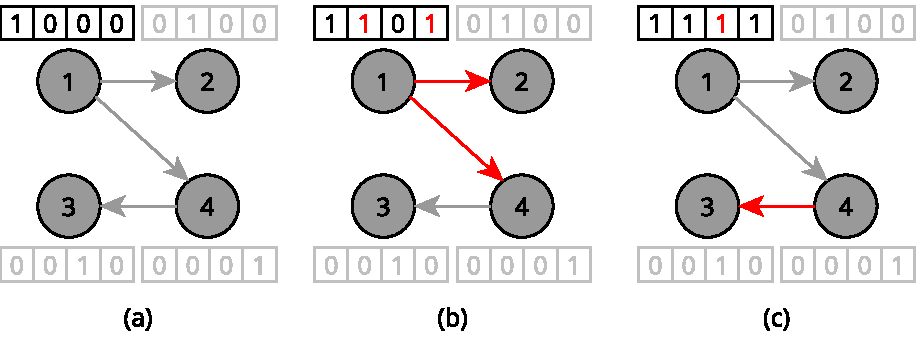
\includegraphics[width=0.85\linewidth]{images/infuserdiff.pdf}
    \caption{{\sc InFuseR} diffusion process illustrated for \emph{only vertex $1$} on toy sample graph.  (a) \label{fig:infuserinit} Toy graph InFuseR initialization.  (b) \label{infuserdiff1} First level of diffusion using \emph{push-based} method for vertex $1$. (c) Second level of diffusion following Fig.\ref{fig:infuserdiff}(a).
     }\label{fig:infuserdiff} 
    \end{center}
\end{figure}

After the diffusion process, the following steps are repeated until $K$ vertices are added to the seed set $S$. First, for each $v \in V$, the cardinality of the reachability set, $R_G(S \cup \{v\})$, is estimated by merging $M_{S'}$ and $v$'s sketch registers where $M_{S'}$ is the set of sketch registers for the seed set $S$ used to estimate the number of already influenced vertices by $S$\footnote{In fact, the definition is exact only if the error-adaptive, smart sketch rebuilding is disabled. As it will be described in the following subsection, when \acro's error-adaptive mechanism is enabled, $M_{S'}$ is periodically rebuilt to estimate the cardinality of reachability sets over the remaining, unblocked vertices. This is why $S'$ is used instead of $S$.}. Before the kernel, these registers are initialized with zeros. Second, a vertex $s$ with the maximum cardinality estimation is selected and added to $S$. Third, the actual simulations are performed to compute the reachability set of $S$. Having an actual $R_G(S)$ allows us to calculate the estimation errors and find the blocked vertices for all simulations, which is vital since these blocked vertices can be skipped during the next diffusion steps. Besides, we leverage the actual influence to have an {\em error-adaptive kernel}, i.e., to compute the actual sketch error and rebuild the sketches when the accumulated error reaches a critical level which can deteriorate the quality for the following seed vertex selections.

\subsubsection{Error-adaptive sketch rebuilding}

Sketches are fast. However, each sketch operation, including update and merge, can decrease their estimation quality below a desired threshold. Our preliminary experiments revealed that sketches are highly competent at finding the first few seed vertices for influence maximization. Unfortunately, after a few seed vertices, the values inside the sketch registers $M_{S'}$, which are updated at line~\ref{line:if} of Algorithm~\ref{algo:main} via merging with new seed vertex $s$'s reachability set, become large. The saturation of $M_{S'}$ registers is important since \acro uses them to select the best seed candidate at line~\ref{line:estimate}. When they lose their sensitivity for seed selection, a significant drop in the quality is observed. 

\begin{figure}[!ht]
    \begin{center}
    \includegraphics[width=\linewidth]{images/sketch-saturation.pdf}
    \caption{ Effect of register saturation on {\tt Amazon0302} dataset using \acro(${\cal J}=256$) without rebuilding against Greedy($\mathcal{R}=20000$) method\cite{kempe2003maximizing}. %\kktodo{buna TIMS'in sonuclarini da ekleyebilir miyiz - en kaliteli o diye, eger mavinin ustunde kaliyorsa guzel} \ggx{Bunun için süreye ihtiyacım var. Diğer algorithmlar mavi çizgi gibi olmalı,(SKIM hariç) 
     }\label{fig:sketch-saturation} 
    \end{center}
\end{figure}


% \begin{figure*}[!ht]
%     \begin{center}
%         \subfloat[{\tt LiveJournal} execution time in seconds\label{fig:lj-time}]{%
%         \includegraphics[width=0.48\linewidth]{images/heatmap_LiveJournal_time.pdf}
%     }
%     \subfloat[{\tt Orkut} execution time in seconds\label{fig:Orkut-time}]{%
%         \includegraphics[width=0.48\linewidth]{images/heatmap_Orkut_time.pdf}
%         }
%     \subfloat[{\tt Pokec} execution time in seconds\label{fig:Pokec-time}]{%
%         \includegraphics[width=0.48\linewidth]{images/heatmap_Pokec_time.pdf}
%         }\\
%         \subfloat[{\tt LiveJournal} influence score\label{fig:lj-score}]{%
%         \includegraphics[width=0.48\linewidth]{images/heatmap_LiveJournal_score.pdf}
%         }
%     \subfloat[{\tt Orkut} influence score\label{fig:Orkut-score}]{%
%         \includegraphics[width=0.48\linewidth]{images/heatmap_Orkut_score.pdf}
%         }
%     \subfloat[{\tt Pokec} influence score\label{fig:Pokec-score}]{%
%         \includegraphics[width=0.48\linewidth]{images/heatmap_Pokec_score.pdf}
%         }\\
%     \end{center}
%     \caption{Effect of $\epsilon$ parameters on \acro(${\cal J} = 256$, $\epsilon_c=0.02$) performance, using $\tau=16$ threads. Lighter shades are better. }\label{fig:parameter-smallmultiples} 
% \end{figure*}    
%\begin{figure}[ht] 
%    \centering
%    \includegraphics[width=1\linewidth]{images/converge-performance.pdf}
%  \centering \caption{Geometic mean of \acro's performance and results quality on different $\epsilon_c$ parameters (${\cal J}=256,\epsilon_l=0.3,\epsilon_g=0.01,\tau=18$) \kktodo{bu alttaki figurlerde sagdaki degerler sanki ters - kirmizi siyah bu sekilde mi siralanmali}. 
%    \label{fig:conv-perf}} 
%\end{figure}


Figure~\ref{fig:sketch-saturation} shows the effect of register saturation by comparing two \acro variants; the first one rebuilds a new sketch to choose each seed vertex $s$, i.e., the {\bf else} part in lines~\ref{line:else1}--\ref{line:else2} of Algorithm~\ref{algo:main} is executed for every iteration of the {\bf for} loop at line~\ref{line:for}. This sketch is built on the residual graph $G \setminus R_G(S)$, which remains after the current seed set's reachability is removed. The second variant builds a  sketch only once at the beginning and employs it through the IM kernel, i.e., the {\bf else} part is never executed. The figure shows that the latter's seed selection quality is comparable to that of the former for the first few seed vertices. However, a significant reduction in the quality is observed for the later vertices. Furthermore, the former approach's quality is on par with the expensive Greedy algorithm's quality, which computes actual reachability sets. This shows that sketch-based estimation can perform as well as the accurate but expensive approach. Note that rebuilding also allows \acro to work on a smaller problem for the following seed vertex selection since we remove the already influenced vertices from sample subgraphs and work on the remaining subgraphs. %Hence, for the remaining estimations, we only need to consider {\em latent} seed vertices of $S$, which are chosen after the sketch rebuild.



Although its quality is on par with the traditional algorithm, the variant which rebuilds a sketch for all the seed vertex selections can be expensive. Here, we leverage an error-adaptive approach by rebuilding them when a significant cardinality estimation error is observed. 
%As After adding vertices to the seed set, \acro performs Monte-Carlo simulations to estimate the reachability of the latent seed set.
The estimation error is calculated as follows; we store the influence score after each sketch rebuild in $\varsigma$~(line~\ref{line:else2} of Algorithm~\ref{algo:main}). Let $\sigma$ be the real influence for the seed set $S$ including the selected vertex. We first compute the marginal influence gain $\delta = \sigma - \varsigma$, which is the additional influence obtained since the last sketch rebuilt. Note that $e$, computed at line~\ref{line:e} is the sketch estimate for this value. \acro computes the local estimation error $err_l = |(e-\delta) / \delta|$ and the global error $err_g=|(e-\delta) / \sigma|$. The sketches are assumed to be fresh if 
the local estimation error $err_l$ is smaller than a local threshold $\epsilon_{l}$ or the global error $err_g=|(e-\delta) / \sigma|$ is smaller than a global threshold $\epsilon_{g}$.

%Before rebuilding stale sketches, the reachability set of the latent seed set, $R_G(S')$, is marked as visited and considered blocked in their respective simulations while rebuilding the sketches. Then, the sketches are rebuilt using Monte-Carlo simulations. After rebuilding, $M_{S'}$, which holds the seed vertices' cardinality estimate added after the last rebuild, is cleared with all zeros.
 
%This approach allows us to keep the sketches in high quality even after many vertices are added to the seed set. But on the other hand, it forces us to perform expensive Monte-Carlo simulations. 
%We reuse the reachability sets of the latent seed set, $R_G(S')$, computed by Monte-Carlo simulations. While rebuilding the sketches, $R_G(S')$ is used to check whether a vertex is blocked in a sample.

%Other methods mentioned in this paper do not report the time spent on calculating the influence scores, whereas our approach includes the time since it is crucial for keeping the sketches in high quality.


\begin{figure*}[!ht]
    \begin{center}
        \subfloat[{\tt LiveJournal} execution time in seconds\label{fig:lj-time}]{%
        \includegraphics[width=0.33\linewidth]{images/heatmap_LiveJournal_time.pdf}
    }
    \subfloat[{\tt Orkut} execution time in seconds\label{fig:Orkut-time}]{%
        \includegraphics[width=0.33\linewidth]{images/heatmap_Orkut_time.pdf}
        }
    \subfloat[{\tt Pokec} execution time in seconds\label{fig:Pokec-time}]{%
        \includegraphics[width=0.33\linewidth]{images/heatmap_Pokec_time.pdf}
        }\\
        \subfloat[{\tt LiveJournal} influence score\label{fig:lj-score}]{%
        \includegraphics[width=0.33\linewidth]{images/heatmap_LiveJournal_score.pdf}
        }
        \subfloat[{\tt Orkut} influence score\label{fig:Orkut-score}]{%
        \includegraphics[width=0.33\linewidth]{images/heatmap_Orkut_score.pdf}
        }
    \subfloat[{\tt Pokec} influence score\label{fig:Pokec-score}]{%
        \includegraphics[width=0.33\linewidth]{images/heatmap_Pokec_score.pdf}
        }
    \end{center}
    \caption{Effect of $\epsilon$ parameters on \acro(${\cal J} = 256$, $\epsilon_c=0.02$) performance, using $\tau=16$ threads. Lighter shades are better. }\label{fig:parameter-smallmultiples} 
\end{figure*}    

The use of two different, local and global, thresholds allows the algorithm to rebuild the sketches after significant local errors and skip this expensive process if the estimation error is insignificant compared to the total influence. As explained above, when the rebuilding is skipped, \acro only updates $M_{S'}$ by merging it with the candidate vertex's sketch. Hence, the selected threshold values, $\epsilon_{l}$ and $\epsilon_{g}$, have a significant impact on the performance. In the setting $\epsilon_{l} = \epsilon_{g} = 0$, the algorithm always rebuilds. Conversely, setting $\epsilon_l = \epsilon_{g} = \infty$ will make \acro fast since sketches are built only once. However, the influence scores will suffer, which is already shown by Fig.~\ref{fig:sketch-saturation}. To evaluate the interplay and find the thresholds that yield a nice tradeoff, we conducted a grid search in which \acro's execution time and influence quality are measured for different parameters. The results of this preliminary experiment are shown in Figure~\ref{fig:parameter-smallmultiples}.  We found that the parameters $\epsilon_{l}=0.3$ and $\epsilon_{g}=0.01$ perform well on many datasets, both in terms of speed and quality. %For these experiments, $\epsilon_c = 0.02$ is used.

% \subsection{Correctness of \acro{}} 
% The greedy solution for influence maximization is well studied and proven to be correct~\cite{kempe2003maximizing}. \acro uses the same optimization method but replaces reachability set computations with sketches instead of per-vertex graph traversal and labeling. Since only the reachability set computations are different, we will comment on the correctness of the sketches used.

% Flajolet-Martin sketches processes elements in a stream to estimate distinct elements observed; for reachability set computations, instead of a stream, we process a spanning tree on the sampled graph. Instead of adding the elements one by one, sketches that are connected is merged. This operation is identical to processing a spanning-tree in a sampled subgraph in parallel. The FM sketches used only store the maximum leading zero counts which are merged by taking the maximum of two where the {\tt max} operation is associative. \acro processes one level of depth at each iteration, and the maximum value observed is updated for each vertex. Assume that we have a toy graph with 3 edges, ($a\to b, a \to c, c \to d$); a sequential traversal  observes $a$, $b$, $c$, $d$ in order so $M[a] = max(max(max(a, b), c), d)$. On the other hand, our method pulls values from incoming edges $M[a] = max(max(a,b), max(c,d))$. Both methods produce the same results; $M[a] =max(max(max(a, b), c), d)=max(max(a,b), max(c,d))$.

\subsection{Runtime Analysis}\label{sec:runtime}

The seed selection process requires $K$ iterations to select $K$ seed vertices. For a single iteration, we have multiple steps each processing a single depth of information, e.g., neighborhood. The propagation process is actually a reverse influence process that starts with whole graph as frontier and diffuses register values with respect to the sample graphs. In the worst case, i.e., assuming all edges are processed and all the sketch registers are updated at each step, each iteration of the seed-set construction has ${\mathcal O}(d \times (|V|\times \mathcal{J} + |E|))$ time complexity where $d$ is the diameter of $G$ which is the number of steps at each iteration. However, on average, a single iteration of \acro performs much faster. First, as explained above, $d$ is a loose upper bound on the number of steps. Second, since only the recently updated registers are propagated to the next step, and only the edges in a sample are processed, a small fraction of the graph is processed for each step. Last, the complexity reduces for later iterations, since the nodes and their edges, which are already covered by the reachability set of the current seed set, are not processed. 

These analysis and observations tell us that when the probability of being influenced, i.e., the average probability of an edge being in a sampled subgraph, is high, the samples will be denser and hence, the actual number of steps \acro performs will be smaller. Furthermore, depending on the topology of $G$, the marginal influence scores of the first few vertices can be much higher with larger probability values and adding these vertices to the seed set will leave less number of vertices to be processed for later iterations. On the other hand, increasing the influence probabilities also increase the number of edges to be processed on the samples. Note that other factors that has an impact on the overall performance exist such as the number of iterations skipping the sketch rebuilding. This also depends on $G$'s structure as well as the influence probabilities. Still, as the experiments also will show, \acro's execution time tends to decrease for many graphs when the influence probabilities increase.

%  


% \begin{equation}
%  sketch-union-chance for \alpha-bit sketch = \frac{1}{2^{\alpha+1}}  \frac{2^{\alpha}-1}{2^\alpha}
% \end{equation} 


% \begin{equation}
%     \label{eq:activeverts}
%     \begin{array}{l}
%     A_0 = N\\
%     A_t = \(\sum_{v \in V}^{} 1-(1-(0.32*A_{t-1}/N)^{p|\Gamma(v)|} \)\\
%     % \mathcal{O}(max(\Gamma({A_t}), TN))
%     \end{array}
% \end{equation} 

% Sum[Divide[1,\(40)Power[2,\(40)a+1\(41)]\(41)]Divide[Power[2,a]-1,Power[2,a]],{a,0,6}]

\subsection{Approximation Ratio of \acro} 

The influence function is non-negative, monotone, and sub-modular; hence, adding a single vertex to the current seed set can only increase the overall influence and decreases the marginal influence scores for the remaining vertices that are not in the set. A greedy solution of final size $K$ is at least $1-(1-1/K)^K \approx 63.5\%$ of the optimal solution~\cite{nemhauser1978analysis}. Since it uses sketches, \acro's approximation guarantee is not straightforward to derive. This being said, based on the average approximation performance of the sketches, we can argue the following. \acro is a greedy algorithm; vertices with a maximum reachability which is estimated via sketches. At each iteration, \acro can choose a vertex worse than the local optimum due to its estimation errors. Since the standard error for the FM sketch is $~1.30/\sqrt{\mathcal{J}}$~\cite{durand2003loglog}, we can expect $(1-1.3/\sqrt{256}) \times (1-(1-1/50)^{50}) \approx 58.4\%$ of the optimal solution for $K = 50$ and $\mathcal{J} = 256$. However, as the greedy algorithm, the practical performance is better. Furthermore, the mistakes in previous iterations can be rectified in later iterations due to submodularity.

\subsection{Implementation Details}
%\subsection{Regularization and Vectorization}
%Sampled edges are stored together, diffusion related information stored afar. This way, SIMD operation is allowed on consecutively located edges, requiring random memory accesses for the diffusion process. Even if the sample or diffusion information are stored closely, without fusing, the random access overhead will be still there and much memory will be wasted. 

%One of the main advantages of fused sampling is allowing similar simulation data and computations together. For processing samples for an edge in algorithm \ref{algo:diffusion-step}~(lines~\ref{ln:inner_start}--\ref{ln:inner_end}).  

To efficiently process real-life graphs, \acro uses the Compressed Sparse Row~(CSR) graph data structure.\fixme{ In CSR, an array, $ptrs$, holds the starting indices} of the adjacency lists for each vertex, while \fixme{another} array, \fixme{$adj$, holds} the actual adjacency lists (i.e., the outgoing neighbors) one after another. Hence, the adjacency list of vertex $i$ is located in $adj$ at locations $adj[ptrs[i], \ldots, ptrs[i+1] - 1]$. 
    
The traditional two-step (sample-then-diffuse) computation model stores the (graph) data in a loosely coupled fashion.
% That is the data is clustered w.r.t. their simulation IDs. 
While designing \acro, we fine-tuned it to be vectorization friendly, including its data layout and computation patterns. These design choices allow us to perform multiple operations, i.e., the same operations but on different data, at once. For instance, we keep all the memory registers of a single vertex from different simulations adjacent, and this allows the efficient use of vectorized computation hardware while performing lines~\ref{ln:vec1}--\ref{ln:update} of Algorithm~\ref{algo:diffusion-step}. Also, random number generation, fused sampling, and sketch merging are vectorizable operations when the data are stored in a coupled way as in \acro.
%Vectorization also reduces branching on the overall computation; When vectorized, many comparison operations are done without branching. 
%%%%%%%%%%%%%%%NEW

We allow a single easy-to-predict branch after the sample edges are generated to exit early without merging the registers. In our experiments, sorting random values $X_r$ significantly increases the performance by clustering similar simulations together while preserving branch locality. Since sorted random values are XOR'ed with the same edge hash values, it is more likely to non-taken edges are sampled together. For example, the naive approach has only $13\%$ vector units filled while processing Amazon dataset with $0.01$ edge probabilities. Sorting the $X_r$ values increases the fill rate  $32\%$. This shows that, the early-exit branch is taken $2.4\times$ more, reducing the total number of arithmetic operations from $23$ to $9$ per edge traversal.

% Up to 20\% speed-up can be achieved by an early exit at line \ref{ln:early_exit} using sorted random values.   
Multi-thread parallelization is achieved using OpenMP pragmas; the sketch computation and Monte-Carlo simulations are performed in per-vertex tasks. This approach allow us to preserve both temporal and spatial locality. The OpenMP tasks are distributed to the threads via dynamic scheduling with large enough chunks~(8192) to mitigate scheduling costs. Even though dynamic scheduling has a higher cost than the static scheduling, it is preferable due to uneven edge distribution among the vertices of $G$ (as well as of the sampled subgraphs).  

\acro computes the actual influence via an iterative processing of the vertices' neighborhoods starting with a queue containing the seed set. This approach allows multiple threads to process different vertices at the same time. The visited vertices are labeled in parallel without any synchronization since the operations are idempotent, and they can be done simultaneously in any order. In addition, we utilize SIMD vectors to process multiple samples simultaneously for each thread. This approach is wasteful for small influence graphs, but the error-adaptive rebuilding strategy allows us to mitigate the cost in such conditions.   

%%%%%%%%%%%%%%%%%%%%%%%%%NEW END
\section{Experimental Results}\label{sec:evaluation}
We performed the experiments on a server with an 16-core {\tt Intel Xeon E5-2620 v4} CPU, running at 2.10GHz, and 192GB memory. The Operating System on the server is {\tt Ubuntu 20.04.2 LTS} with  5.4.0-65 kernel. The algorithms are implemented using {\tt C++20}, and compiled with {\tt GCC 9.3.0} with {\tt "-Ofast"} and {\tt "-march=native"} optimization flags. Multi-thread parallelization was achieved with {\tt OpenMP} pragmas. {\tt AVX2} instructions are utilized by handcrafted code with vector intrinsics.
\\

\begin{table}[!ht]
\caption{Properties of networks used in the experiments}\label{tab:NetProps}
\centering
% \scalebox{0.95}{
\resizebox{1\columnwidth}{!}{
\begin{tabular}{ll||r|r|r|r}
& & No. of           & No. of    & Avg.  & Diameter\\
&Dataset & Vertices          & Edges           &  Degree               \\
\hline
\multirow{3}{*}{\scriptsize\rotatebox[origin=c]{90}{Undirected}}& {\tt Amazon0302} & 262,113 & 1,234,878 & 4.71 & 32\\
&{\tt DBLP} & 317,081 & 1,049,867  & 3.31 & 21\\
% &{\tt NetHEP} & 15,235 & 58,892 & 1.83 & 3.87 \\
% &{\tt NetPhy} & 37,151 & 231,508 & 1.28 & 6.23 \\
&{\tt Orkut} & 3,072,441 & 117,185,083& 38.14 & 9\\
&{\tt Youtube} & 1,134,891 & 2,987,625  & 2.63 & 20\\

\hline
\multirow{6}{*}{\scriptsize\rotatebox[origin=c]{90}{Directed}}&{\tt Epinions} & 75,880 & 508,838  & 6.71 & 14\\
&{\tt Friendster} & 65,608,366 & 1,806,067,135  & 27.53 & 32\\
&{\tt LiveJournal} & 4,847,571 & 68,993,773  & 14.23 & 16\\
&{\tt Pokec} & 1,632,803 & 30,622,564  & 18.75 & 11\\
&{\tt Slashdot0811} & 77,360 & 905,468  & 11.70 & 10\\
&{\tt Slashdot0902} & 82,168 & 948,464  & 11.54 & 11\\
% &{\tt Twitter} & 81,306 & 2,420,766 & 1.37 & 29.77 
\end{tabular}
}
\end{table}
% \FloatBarrier
\subsection{Experimental Settings} \label{sec:expset}

We performed the experiments on ten graphs~(four undirected, six directed). For comparability, graphs that have been frequently used within the Influence Maximization literature are selected. The properties of these graphs are given in Table~\ref{tab:NetProps}:  {\tt Amazon0302} is an Amazon co-purchase network, {\tt DBLP} is DBLP collaboration network, {\tt Orkut} is an online social network where users form friendship,  {\tt Youtube} is a video social video sharing platform that allows friendship relations, {\tt Epinions} is a consumer review trust network, {\tt Friendster} is a social gaming website where users can form friendship edge each other, {\tt LiveJournal} is a blogging site that allows users to add friends, {\tt Pokec} is the Slovakian poker game site friend network, and {\tt Slashdot} networks are friend-foe networks~(08-11, 09-11).

Five diffusion settings are simulated for a comprehensive experimental evaluation; for each network, we use 
\fixme{
\begin{enumerate}
  \setlength{\itemsep}{0.2pt}
  \setlength{\parskip}{0pt}
  \setlength{\parsep}{0pt}
    \item constant edge weights $w = 0.005$,
    \item constant edge weights $w = 0.01$~(as in~\cite{kempe2003maximizing} and~\cite{MixGreedy}),
    \item constant edge weights $w = 0.1$~(as in~\cite{kempe2003maximizing}),
    \item normally distributed edge weights $w \in N(0.05,0.025)$,
    \item uniform distributed edge weights $w \in U(0,0.1)$.
    % \item weighted cascade edge weights $w_{u,v} = 1/|\Gamma(v)|$.
\end{enumerate}
}
\noindent We selected $w=0.005$ as a setting to challenge \acro. As explained in Section~\ref{sec:runtime}, due to the nature of its diffusion algorithm, \acro is expected to perform slower on sparser samples. The later two settings, i.e., $w = 0.01$  and $w = 0.1$, are selected to emulate the experiments of~\cite{kempe2003maximizing} and~\cite{MixGreedy}. In addition to constant edge weights, we performed experiments on two different statistical distributed edge weights to test how algorithms behave on mixed (large and small edge weights together) edge weights. The normal distribution setting incurs a small number of extreme sketch values and uniform distribution setting incurs a large number of large sketch values.

\subsection{Performance Metrics}

The algorithms are evaluated based on (1) execution time, (2) influence score, and (2) maximum memory used. For Influence Maximization, there is a trade-off among these performance metrics; in one extreme, it is trivial to select random vertices as the seed set. In another, one can compute the reachability sets of every possible seed set of size $K$ and choose the best one. 
%The observed execution times and memory consumption of different algorithms are comparable when the algorithms run on the same computer.
In all our experiments, the execution times are the wall times reported by the programs. All the methods we benchmarked exclude the time spent on reading files and preprocessing. %We only left out the time to spend on reading files for \acro. 
We allowed all methods to utilize the given number of CPU cores in all benchmarks, except {\sc Tim+}, which is a single-threaded algorithm. The memory use reported in this paper is the {\em maximum resident set sizes}~(RSS), which are measured using GNU {\tt time} command.

Since the algorithms may use different methods to measure the influence, the reported influence scores may not be suitable for comparison purposes with high precision. Due to this reason, we implemented an independent oracle with a straightforward, sample-then-diffuse algorithm without any optimizations. For sampling, the random values are generated by the 32-bit Mersenne Twister pseudo-random generator {\tt mt19937} from {\tt C++} standard library. This algorithm-independent oracle obtains all the influence scores in this paper.

\subsection{Algorithms evaluated in the experiments}

We evaluated our method against four other state-of-the-art influence maximization algorithms, {\sc Tim+}, {\sc Skim}, {\sc Ripples}, and {\sc Ssa}. The first algorithm focuses on the influence score, whereas the second is a sketch-based algorithm that takes the execution time into account. The third one is a scalable, parallel approximation algorithm with a parameter to control the influence quality, and the last one leverages a Stop-and-Stare strategy.

\begin{itemize} [leftmargin=0.3cm]
\item The Two-phased Influence Maximization~({\sc Tim+}) runs in two phases: {\em Parameter Estimation} which estimates the maximum expected influence and a parameter $\theta$ and {\em Node Selection} which randomly samples $\theta$ reverse reachability sets from $G$ and then derives a size-$K$ vertex-set $S$ that covers a large number of these sets~\cite{tim}. The algorithm has a parameter $\epsilon$ which allows a trade-off between the seed set quality and execution time. In our experiments, we set  $\epsilon=0.2$ to have a high-quality influence maximization baseline as suggested by the software. We also experimented with $\epsilon = 1.0$ as authors' suggested, which gives around $8\times$ speedup on average but a reduction on the influence score up to $9\%$.

\item The Sketch-based Influence Maximization~({\sc Skim}) uses a combined bottom-$k$ min-hash reachability sketch~\cite{bottomk} to estimate the influence scores of the seed sets~\cite{cohen2014sketch}. As suggested by the authors, in this work, we employ {\sc Skim} with $k = 64$ and $\ell = 64$ sampled subgraphs. The implementation (from the authors) is partially parallelized and leverages multicore processors. However, it  assumes a constant $w$ value; hence, we only used {\sc Skim} for the first three settings given in Section~\ref{sec:expset}.

\item Minutoli et al.'s {\sc Ripples} is a high-performance, parallel algorithm that efficiently produces accurate seed sets~\cite{minutoli2019fast}. 
It is an approximation method that improves the Reverse Influence Sampling~(RIS)~\cite{borgs2014maximizing} algorithm by eliminating the need for the threshold to be used. %{\sc Ripples} generalizes the influence of all vertices on a small set of sample graphs that is sampled from the reachability sets of a few vertices. 
We have used $\epsilon = 0.5$ as suggested in the original paper, where $\epsilon$ is a user-defined parameter to control the approximation boundaries.

\item Nguyen et al. proposed {\sc Ssa} and {\sc D-Ssa}~\cite{nguyen2016stop}, two novel sampling approaches for Influence Maximization problem. {\sc Ssa} and its dynamic network variant {\sc D-Ssa} are fast methods compared to previously mentioned approaches while providing similar approximation guarantees. The approach employs a novel Stop-and-Stare strategy. It stops at exponential checkpoints to verify (stare) if there is adequate statistical evidence on the solution quality. We used {\sc Ssa} for our benchmarks since our networks are static. 


\end{itemize}
%Finally, our method \acro employs both Monte-Carlo simulations and count-distinct sketches for estimating reachability set cardinalities. Even though \acro is blazing-fast and accurate for limited $K$, we exploit the performance of the method to improve the results by rebuilding sketches after removing residual influence networks.











%%%%%%%%%%%%%%%%%%%%%%%%%%%%%%%%%%%%%%%%%%%%%%%%%%%%%%%%%%%%%%%%%%%%%%





%%%%%%%%%%%%%%%%%%%%%%%%%%%%%%%%%%%%%%%%%%%%%%%%%%%%%%%%%%%%%%%%%%%%%%


% \begin{table*}
%     \setlength{\tabcolsep}{1.2pt}
%         \caption{\acro execution times~(in secs), influence scores, and memory use~(in GBs)  on the networks with $K = 50$ seeds using $\tau=16$ threads and constant edge weights $w=0.005$. Influence scores are given relative to \acro{}. The runs that did not finish in 5 hours or due to high memory use shown as "-".
%         }
%         \label{tab:timings0.005}
%         \centering
%         \resizebox{\linewidth}{!}{
    
% \begin{tabular}{l|rrrrrr|rrrrrr|rrrrrr}
% \toprule
% {} & \multicolumn{6}{c|}{Time} & \multicolumn{6}{c|}{Score} & \multicolumn{6}{c}{Memory} \\
% Method & \multicolumn{2}{c}{{\sc \acro}} &   {\sc Tim+} &    {\sc Ripples} &    {\sc Skim} &     {\sc Ssa} & \multicolumn{2}{c}{{\sc \acro}} &    {\sc Tim+} &     {\sc Ripples} &    {\sc Skim} &     {\sc Ssa} & \multicolumn{2}{c}{{\sc \acro}} &  {\sc Tim+} &  {\sc Ripples} &   {\sc Skim} &  {\sc Ssa} \\
% R &        256 &     512 &    0.2 &    0.5 &   64-64 &     0.1 &        256 &        512 &     0.2 &     0.5 &   64-64 &     0.1 &        256 &    512 &   0.2 &  0.5 &  64-64 &  0.1 \\
% Dataset                 &            &         &        &        &         &         &            &            &         &         &         &         &            &        &       &      &        &      \\
% \midrule
% \tt{Amazon0302}              &       2.18 &    3.99 & 295.32 &  64.45 &   12.69 &   11.40 &      96.19 &       99.1 &  1.023x &  0.998x &  0.557x &  0.988x &       0.10 &   0.18 & 45.03 & 1.01 &   1.51 & 1.35 \\
% \tt{DBLP}                &       2.92 &    4.39 & 480.22 &  64.91 &   13.18 &   28.40 &     107.86 &      111.7 &  1.017x &  0.967x &  0.977x &  0.996x &       0.16 &   0.27 & 66.98 & 1.05 &   1.38 & 2.68 \\
% \tt{Friendster}          &    1088.25 & 1775.58 &      - &      - & 4055.92 &       - & 4942827.00 &  4942856.5 &       - &       - &  1.000x &       - &      88.94 & 122.42 &     - &    - & 112.33 &    - \\
% \tt{Orkut}               &      39.38 &   69.93 &      - & 253.44 &   49.02 & 1245.28 &  158915.22 &   158994.0 &       - &  0.997x &  1.001x &  0.995x &       4.36 &   5.18 &     - & 7.97 &   1.77 & 5.81 \\
% \tt{Youtube}             &       5.40 &    7.59 &  82.08 &  63.71 &    5.67 &    3.76 &    1827.39 &     1834.4 &  1.023x &  1.010x &  1.005x &  1.009x &       0.42 &   0.73 &  7.41 & 0.63 &   0.53 & 0.37 \\
% \tt{Epinions}           &       1.79 &    2.84 &  13.61 &  47.93 &    1.86 &    0.58 &     238.65 &      241.7 &  1.009x &  0.973x &  0.986x &  0.965x &       0.03 &   0.05 &  3.70 & 0.24 &   0.17 & 0.10 \\
% \tt{LiveJournal}        &      15.02 &   26.13 & 684.52 &  74.62 &   22.28 &   16.98 &    5559.85 &     5748.5 &  1.030x &  1.015x &  1.005x &  1.006x &       2.40 &   3.70 & 17.06 & 2.19 &   2.05 & 1.38 \\
% \tt{Pokec} &      13.21 &   21.63 & 312.19 &  78.59 &   23.19 &   16.85 &     588.87 &      594.2 &  1.012x &  0.985x &  0.984x &  0.978x &       0.92 &   1.36 & 33.18 & 1.80 &   1.78 & 1.09 \\
% \tt{Slashdot0811}        &       2.02 &    3.64 &  12.83 &  38.49 &    1.34 &    1.02 &     326.32 &      328.1 &  1.017x &  1.000x &  0.987x &  0.989x &       0.04 &   0.06 &  2.47 & 0.20 &   0.13 & 0.10 \\
% \tt{Slashdot0902}        &       1.86 &    3.10 &  14.87 &  38.17 &    1.41 &    0.47 &     338.85 &      341.5 &  1.017x &  0.987x &  0.992x &  0.978x &       0.04 &   0.06 &  2.66 & 0.21 &   0.13 & 0.06 \\
% \bottomrule

% Avg. Perf.&0.61x&1.00x&31.00x&9.91x&1.33x&3.30x&0.99x&1.00x&1.02x&0.99x&0.95x&0.99x&0.66x&1.00x&87.14x&2.79x&2.50x&2.78x \\
% Max. Perf.&0.71x&1.00x&109.39x&16.88x&3.18x&17.81x&1.00x&1.00x&1.03x&1.02x&1.01x&1.01x&0.84x&1.00x&257.27x&5.76x&8.64x&9.93x \\
% Geo. Mean&0.61x&1.00x&15.09x&8.19x&1.01x&0.96x&0.99x&1.00x&1.02x&0.99x&0.94x&0.99x&0.65x&1.00x&41.46x&2.19x&1.59x&1.51x \\
% \end{tabular}
% }\end{table*}
% \begin{table*}
%     \setlength{\tabcolsep}{1.2pt}
%         \caption{\acro execution times~(in secs), influence scores, and memory use~(in GBs)  on the networks with $K = 50$ seeds using $\tau=16$ threads and constant edge weights $w=0.01$. Influence scores are given relative to \acro{}. The runs that did not finish in 5 hours or due to high memory use shown as "-".
%         }
%         \label{tab:timings0.01}
%         \centering
%         \resizebox{\linewidth}{!}{
    
% \begin{tabular}{l|rrrrrr|rrrrrr|rrrrrr}
% \toprule
% {} & \multicolumn{6}{c|}{Time} & \multicolumn{6}{c|}{Score} & \multicolumn{6}{c}{Memory} \\
% Method & \multicolumn{2}{c}{{\sc \acro}} &    {\sc Tim+} &    {\sc Ripples} &    {\sc Skim} &     {\sc Ssa} & \multicolumn{2}{c}{{\sc \acro}} &    {\sc Tim+} &     {\sc Ripples} &    {\sc Skim} &     {\sc Ssa} & \multicolumn{2}{c}{{\sc \acro}} &  {\sc Tim+} &   {\sc Ripples} &  {\sc Skim} &   {\sc Ssa} \\
% R &        256 &     512 &     0.2 &    0.5 &   64-64 &     0.1 &         256 &         512 &     0.2 &     0.5 &   64-64 &     0.1 &        256 &    512 &   0.2 &   0.5 & 64-64 &   0.1 \\
% Dataset                 &            &         &         &        &         &         &             &             &         &         &         &         &            &        &       &       &       &       \\
% \midrule
% \tt{Amazon0302}              &       1.62 &    2.74 &  211.25 &  52.76 &   12.48 &    7.33 &      155.81 &       156.8 &  1.009x &  0.978x &  0.393x &  0.991x &       0.10 &   0.18 & 35.22 &  0.67 &  1.43 &  0.70 \\
% \tt{DBLP}                &       2.03 &    2.05 &  145.54 &  59.23 &    7.36 &   13.95 &      232.12 &       234.7 &  1.027x &  1.002x &  0.978x &  1.006x &       0.16 &   0.27 & 24.53 &  0.61 &  0.82 &  1.38 \\
% \tt{Friendster}          &     902.78 & 1334.65 &       - &      - & 2641.58 &       - & 11504743.00 &  11504801.0 &       - &       - &  1.000x &       - &      88.94 & 122.42 &     - &     - & 78.17 &     - \\
% \tt{Orkut}               &      46.63 &   73.82 &       - & 606.07 &  125.15 & 5613.07 &   650214.62 &    650243.1 &       - &  1.000x &  1.000x &  1.000x &       4.36 &   5.18 &     - & 20.48 &  3.33 & 27.19 \\
% \tt{Youtube}             &       4.21 &    5.85 & 1056.41 &  50.45 &    8.50 &   19.82 &     9049.47 &      9072.9 &  1.010x &  0.994x &  1.006x &  0.983x &       0.42 &   0.73 & 14.15 &  0.62 &  0.73 &  0.41 \\
% \tt{Epinions}           &       2.20 &    3.80 &   13.13 &  37.47 &    1.17 &    0.35 &      662.66 &       671.8 &  1.007x &  0.982x &  0.995x &  0.982x &       0.03 &   0.05 &  1.51 &  0.17 &  0.11 &  0.04 \\
% \tt{LiveJournal}        &      21.32 &   34.07 &       - &  88.36 &   18.38 &  195.23 &    47272.62 &     47353.7 &       - &  0.995x &  0.999x &  0.990x &       2.40 &   3.70 &     - &  2.96 &  1.47 &  2.52 \\
% \tt{Pokec} &      12.53 &   19.26 &  145.32 &  59.37 &    7.50 &    7.29 &     1843.17 &      1858.2 &  1.015x &  0.985x &  0.979x &  0.988x &       0.92 &   1.36 & 11.43 &  1.12 &  0.76 &  0.61 \\
% \tt{Slashdot0811}        &       2.62 &    5.90 &   39.86 &  35.37 &    1.00 &    1.65 &     1181.84 &      1201.4 &  1.012x &  0.990x &  0.984x &  0.987x &       0.04 &   0.06 &  1.29 &  0.16 &  0.08 &  0.06 \\
% \tt{Slashdot0902}        &       3.09 &    6.29 &   44.51 &  35.27 &    1.12 &    1.00 &     1299.36 &      1305.0 &  1.010x &  0.985x &  0.989x &  0.967x &       0.04 &   0.06 &  1.43 &  0.16 &  0.08 &  0.04 \\
% \bottomrule

% Avg. Perf.&0.64x&1.00x&50.50x&10.24x&1.49x&10.62x&0.99x&1.00x&1.01x&0.99x&0.93x&0.99x&0.66x&1.00x&56.05x&2.33x&1.91x&2.04x \\
% Max. Perf.&0.99x&1.00x&180.58x&28.89x&4.56x&76.04x&1.00x&1.00x&1.03x&1.00x&1.01x&1.01x&0.84x&1.00x&201.20x&3.95x&8.19x&5.24x \\
% Geo. Mean&0.63x&1.00x&19.89x&7.78x&0.83x&1.51x&0.99x&1.00x&1.01x&0.99x&0.90x&0.99x&0.65x&1.00x&32.82x&1.96x&1.23x&1.27x \\
% \end{tabular}
% }\end{table*}
% \begin{table*}
%     \setlength{\tabcolsep}{1.2pt}
%         \caption{\acro execution times~(in secs), influence scores, and memory use~(in GBs)  on the networks with $K = 50$ seeds using $\tau=16$ threads and constant edge weights $w=0.1$. Influence scores are given relative to \acro{}. The runs that did not finish in 5 hours or due to high memory use shown as "-".
%         }
%         \label{tab:timings0.1}
%         \centering
%         \resizebox{\linewidth}{!}{
    
% \begin{tabular}{l|rrrrrr|rrrrrr|rrrrrr}
% \toprule
% {} & \multicolumn{6}{c|}{Time} & \multicolumn{6}{c|}{Score} & \multicolumn{6}{c}{Memory} \\
% Method & \multicolumn{2}{c}{{\sc \acro}} &    {\sc Tim+} &     {\sc Ripples} &    {\sc Skim} &     {\sc Ssa} & \multicolumn{2}{c}{{\sc \acro}} &    {\sc Tim+} &     {\sc Ripples} &    {\sc Skim} &     {\sc Ssa} & \multicolumn{2}{c}{{\sc \acro}} &  {\sc Tim+} &   {\sc Ripples} &  {\sc Skim} &   {\sc Ssa} \\
% R &        256 &    512 &     0.2 &     0.5 &   64-64 &     0.1 &         256 &         512 &     0.2 &     0.5 &   64-64 &     0.1 &        256 &    512 &   0.2 &   0.5 & 64-64 &   0.1 \\
% Dataset                 &            &        &         &         &         &         &             &             &         &         &         &         &            &        &       &       &       &       \\
% \midrule
% \tt{Amazon0302}              &       1.75 &   2.47 &  297.11 &   46.78 &    4.86 &    6.65 &    12072.88 &     12268.8 &  0.991x &  0.973x &  0.786x &  0.941x &       0.10 &   0.18 & 11.26 &  0.37 &  0.54 &  0.20 \\
% \tt{DBLP}                &       0.87 &   1.24 & 2903.95 &   45.21 &    3.84 &   55.24 &    48511.03 &     48528.0 &  1.001x &  0.993x &  1.001x &  0.991x &       0.16 &   0.27 & 69.72 &  1.18 &  0.27 &  1.10 \\
% \tt{Friendster}          &     445.79 & 630.91 &       - &       - & 5660.24 &       - & 36995828.00 &  36995920.0 &       - &       - &  1.000x &       - &      88.94 & 122.42 &     - &     - & 90.95 &     - \\
% \tt{Orkut}               &      16.69 &  24.47 &       - & 1148.06 &  490.06 &       - &  2692305.25 &   2692316.5 &       - &  1.000x &  1.000x &       - &       4.36 &   5.18 &     - & 71.76 & 10.08 &     - \\
% \tt{Youtube}             &       1.84 &   2.57 &       - &   71.50 &   15.78 &  352.45 &   171338.61 &    171374.0 &       - &  0.999x &  1.001x &  0.999x &       0.42 &   0.73 &     - &  4.29 &  1.11 &  5.15 \\
% \tt{Epinions}           &       0.44 &   0.73 &  436.89 &   34.37 &    2.12 &   16.03 &    10463.58 &     10463.0 &  1.004x &  0.996x &  1.004x &  0.995x &       0.03 &   0.05 & 14.77 &  0.37 &  0.18 &  0.36 \\
% \tt{LiveJournal}        &      10.45 &  15.65 &       - &  553.49 &   71.03 &       - &  1683952.25 &   1685214.1 &       - &  0.998x &  1.001x &       - &       2.40 &   3.70 &     - & 46.07 &  1.35 &     - \\
% \tt{Pokec} &       5.08 &   6.65 &       - &  255.79 &   37.06 & 3256.58 &   773994.19 &    774123.9 &       - &  0.999x &  1.001x &  0.999x &       0.92 &   1.36 &     - & 19.60 &  0.99 & 35.56 \\
% \tt{Slashdot0811}        &       0.49 &   0.77 &  994.78 &   33.35 &    3.05 &   31.97 &    23198.49 &     23211.0 &  1.000x &  0.998x &  1.001x &  0.997x &       0.04 &   0.06 & 27.16 &  0.51 &  0.24 &  0.63 \\
% \tt{Slashdot0902}        &       0.53 &   0.91 &  897.28 &   33.07 &    2.89 &   23.58 &    24282.60 &     24294.9 &  1.000x &  0.995x &  1.000x &  0.994x &       0.04 &   0.06 & 26.39 &  0.53 &  0.23 &  0.63 \\
% \bottomrule

% Avg. Perf.&0.68x&1.00x&1067.72x&36.74x&6.04x&109.07x&1.00x&1.00x&1.00x&0.99x&0.98x&0.99x&0.66x&1.00x&293.39x&8.56x&2.03x&9.34x \\
% Max. Perf.&0.76x&1.00x&2341.90x&47.08x&20.03x&489.71x&1.00x&1.00x&1.00x&1.00x&1.00x&1.00x&0.84x&1.00x&451.59x&14.44x&4.01x&26.19x \\
% Geo. Mean&0.67x&1.00x&735.18x&35.56x&4.78x&40.86x&1.00x&1.00x&1.00x&0.99x&0.98x&0.99x&0.65x&1.00x&243.98x&7.42x&1.56x&6.65x \\
% \end{tabular}
% }\end{table*}
% \begin{table*}
%     \setlength{\tabcolsep}{1.2pt}
%         \caption{\acro execution times~(in secs), influence scores, and memory use~(in GBs)  on the networks with $K = 50$ seeds using $\tau=16$ threads and constant edge weights $w \in N(0.05,0.0025)$. Influence scores are given relative to \acro{}. The runs that did not finish in 5 hours or due to high memory use shown as "-".
%         }
%         \label{tab:timingsN0.05}
%         \centering
%         \resizebox{\linewidth}{!}{
    
% \begin{tabular}{l|rrrrr|rrrrr|rrrrr}
% \toprule
% {} & \multicolumn{5}{c|}{Time} & \multicolumn{5}{c|}{Score} & \multicolumn{5}{c}{Memory} \\
% Method & \multicolumn{2}{c}{{\sc \acro}} &   {\sc Tim+} &     {\sc Ripples} &     {\sc Ssa} & \multicolumn{2}{c}{{\sc \acro}} &    {\sc Tim+} &     {\sc Ripples} &     {\sc Ssa} & \multicolumn{2}{c}{{\sc \acro}} &  {\sc Tim+} &   {\sc Ripples} &   {\sc Ssa} \\
% R &        256 &    512 &    0.2 &     0.5 &     0.1 &         256 &         512 &     0.2 &     0.5 &     0.1 &        256 &    512 &   0.2 &   0.5 &   0.1 \\
% Dataset                 &            &        &        &         &         &             &             &         &         &         &            &        &       &       &       \\
% \midrule
% \tt{Amazon0302}              &       1.29 &   1.78 &  27.01 &   43.25 &    1.18 &     1163.06 &      1166.8 &  1.007x &  0.994x &  0.970x &       0.10 &   0.18 &  2.71 &  0.26 &  0.09 \\
% \tt{DBLP}                &       1.37 &   1.80 & 472.64 &   41.12 &   10.69 &     9907.50 &      9959.2 &  1.004x &  0.991x &  0.974x &       0.16 &   0.27 & 13.37 &  0.40 &  0.25 \\
% \tt{Friendster}          &     507.40 & 693.26 &      - &       - &       - & 29459630.00 &  29459654.0 &       - &       - &       - &      88.94 & 122.42 &     - &     - &     - \\
% \tt{Orkut}               &      20.35 &  31.09 &      - & 1158.88 &       - &  2323092.25 &   2323098.8 &       - &  1.000x &       - &       4.36 &   5.18 &     - & 62.48 &     - \\
% \tt{Youtube}             &       1.99 &   2.81 &      - &   65.20 &  231.59 &    86502.31 &     86551.0 &       - &  0.998x &  0.998x &       0.42 &   0.73 &     - &  2.43 &  2.31 \\
% \tt{Epinions}           &       0.78 &   1.16 & 273.44 &   37.02 &    8.23 &     5879.96 &      5880.4 &  1.006x &  0.987x &  0.985x &       0.03 &   0.05 &  7.92 &  0.27 &  0.20 \\
% \tt{LiveJournal}        &      13.77 &  19.94 &      - &  402.54 &       - &   921589.50 &    921552.3 &       - &  0.997x &       - &       2.40 &   3.70 &     - & 26.52 &     - \\
% \tt{Pokec} &       6.48 &   8.95 &      - &  186.87 & 1417.99 &   463128.94 &    463145.3 &       - &  0.998x &  0.998x &       0.92 &   1.36 &     - & 12.00 & 14.09 \\
% \tt{Slashdot0811}        &       0.71 &   0.97 & 549.78 &   39.24 &   22.45 &    13947.56 &     13957.3 &  1.001x &  0.994x &  0.994x &       0.04 &   0.06 & 14.79 &  0.39 &  0.46 \\
% \tt{Slashdot0902}        &       0.72 &   1.08 & 608.24 &   38.43 &   20.22 &    14532.23 &     14548.2 &  1.001x &  0.991x &  0.991x &       0.04 &   0.06 & 16.58 &  0.40 &  0.45 \\
% \bottomrule

% Avg. Perf.&0.71x&1.00x&328.69x&28.52x&42.35x&1.00x&1.00x&1.00x&0.99x&0.99x&0.66x&1.00x&144.08x&5.80x&4.78x \\
% Max. Perf.&0.76x&1.00x&566.78x&40.46x&158.43x&1.00x&1.00x&1.01x&1.00x&1.00x&0.84x&1.00x&261.41x&12.05x&10.38x \\
% Geo. Mean&0.71x&1.00x&197.41x&27.60x&14.84x&1.00x&1.00x&1.00x&0.99x&0.99x&0.65x&1.00x&93.93x&4.73x&3.17x \\
% \end{tabular}
% }\end{table*}
% \begin{table*}
%     \setlength{\tabcolsep}{1.2pt}
%         \caption{\acro execution times~(in secs), influence scores, and memory use~(in GBs)  on the networks with $K = 50$ seeds using $\tau=16$ threads and constant edge weights $w \in U(0,0.1)$. Influence scores are given relative to \acro{}. The runs that did not finish in 5 hours or due to high memory use shown as "-".
%         The runs that did not finish in 5 hours or due to high memory use shown as "-"
%         }
%         \label{tab:timingsU0.1}
%         \centering
%         \resizebox{\linewidth}{!}{
    
% \begin{tabular}{l|rrrrr|rrrrr|rrrrr}
% \toprule
% {} & \multicolumn{5}{c|}{Time} & \multicolumn{5}{c|}{Score} & \multicolumn{5}{c}{Memory} \\
% Method & \multicolumn{2}{c}{{\sc \acro}} &   {\sc Tim+} &     {\sc Ripples} &     {\sc Ssa} & \multicolumn{2}{c}{{\sc \acro}} &    {\sc Tim+} &     {\sc Ripples} &     {\sc Ssa} & \multicolumn{2}{c}{{\sc \acro}} &  {\sc Tim+} &   {\sc Ripples} &   {\sc Ssa} \\
% R &        256 &    512 &    0.2 &     0.5 &     0.1 &         256 &         512 &     0.2 &     0.5 &     0.1 &        256 &    512 &   0.2 &   0.5 &   0.1 \\
% Dataset                 &            &        &        &         &         &             &             &         &         &         &            &        &       &       &       \\
% \midrule
% \tt{Amazon0302}              &       1.35 &   1.79 &  24.34 &   43.84 &    1.16 &     1148.70 &      1149.3 &  1.014x &  0.996x &  0.971x &       0.10 &   0.18 &  2.74 &  0.27 &  0.09 \\
% \tt{DBLP}                &       1.33 &   2.08 & 431.47 &   41.08 &   18.10 &     9863.24 &      9977.6 &  0.999x &  0.981x &  0.980x &       0.16 &   0.27 & 12.64 &  0.39 &  0.38 \\
% \tt{Friendster}          &     479.16 & 720.54 &      - &       - &       - & 29411772.00 &  29411858.0 &       - &       - &       - &      88.94 & 122.42 &     - &     - &     - \\
% \tt{Orkut}               &      20.98 &  31.93 &      - & 1163.91 &       - &  2320279.50 &   2320295.5 &       - &  1.000x &       - &       4.36 &   5.18 &     - & 62.30 &     - \\
% \tt{Youtube}             &       1.97 &   2.76 &      - &   64.23 &  152.21 &    86122.30 &     86140.3 &       - &  0.998x &  0.998x &       0.42 &   0.73 &     - &  2.35 &  2.10 \\
% \tt{Epinions}           &       0.76 &   1.05 & 297.24 &   36.89 &    8.10 &     5830.02 &      5834.5 &  1.006x &  0.987x &  0.982x &       0.03 &   0.05 &  8.63 &  0.27 &  0.18 \\
% \tt{LiveJournal}        &      14.59 &  18.99 &      - &  402.02 &       - &   917259.25 &    917036.2 &       - &  0.997x &       - &       2.40 &   3.70 &     - & 26.39 &     - \\
% \tt{Pokec} &       6.59 &   8.76 &      - &  186.23 & 1220.47 &   461323.28 &    461434.3 &       - &  0.998x &  0.998x &       0.92 &   1.36 &     - & 12.19 & 13.49 \\
% \tt{Slashdot0811}        &       0.65 &   0.91 & 533.28 &   38.76 &   23.31 &    13890.58 &     13903.5 &  1.001x &  0.994x &  0.994x &       0.04 &   0.06 & 12.63 &  0.39 &  0.45 \\
% \tt{Slashdot0902}        &       0.83 &   1.16 & 637.75 &   38.54 &   19.87 &    14490.73 &     14498.4 &  1.001x &  0.991x &  0.991x &       0.04 &   0.06 & 16.90 &  0.40 &  0.45 \\
% \bottomrule

% Avg. Perf.&0.71x&1.00x&327.98x&28.59x&36.32x&1.00x&1.00x&1.00x&0.99x&0.99x&0.66x&1.00x&139.99x&5.80x&4.68x \\
% Max. Perf.&0.77x&1.00x&586.02x&42.60x&139.32x&1.00x&1.00x&1.01x&1.00x&1.00x&0.84x&1.00x&266.19x&12.02x&9.93x \\
% Geo. Mean&0.71x&1.00x&191.45x&27.56x&14.68x&1.00x&1.00x&1.00x&0.99x&0.99x&0.65x&1.00x&92.09x&4.70x&3.25x \\
% \end{tabular}
% }\end{table*}



















% %%%%%%%%%%%%%%%%%%%%%%%%%%%%%%%%%%%%%%%%%%%%%%%%%%%%%%%%%%%%%%%%%%%%%
% \begin{table*}
%     \setlength{\tabcolsep}{1.2pt}
%         \caption{\acro execution times~(in secs), influence scores, and memory use~(in GBs)  on the networks with $K = 50$ seeds using $\tau=16$ threads and constant edge weights $w=0.005$. Influence scores are given relative to \acro{}. The runs that did not finish in 5 hours or due to high memory use shown as "-".
%         }
%         \label{tab:timings0.005}
%         \centering
%         \resizebox{\linewidth}{!}{
    
% \begin{tabular}{l|rrrrr|rrrrr|rrrrr}
% \toprule
% {} & \multicolumn{5}{c|}{Time} & \multicolumn{5}{c|}{Score} & \multicolumn{5}{c}{Memory} \\
% Method & {\sc \acro} &   {\sc Tim+} &    {\sc Ripples} &    {\sc Skim} &     {\sc Ssa} & {\sc \acro} &    {\sc Tim+} &     {\sc Ripples} &    {\sc Skim} &     {\sc Ssa} & {\sc \acro} &  {\sc Tim+} &  {\sc Ripples} &   {\sc Skim} &  {\sc Ssa} \\
% Dataset                 &            &        &        &         &         &            &         &         &         &         &            &       &      &        &      \\
% \midrule
% \tt{Amazon0302}              &       1.99 & 295.32 &  64.45 &   12.69 &   11.40 &       96.5 &  1.047x &  1.021x &  0.571x &  1.014x &       0.09 & 45.03 & 1.01 &   1.51 & 1.35 \\
% \tt{DBLP}                &       2.51 & 480.22 &  64.91 &   13.18 &   28.40 &      107.7 &  1.046x &  1.008x &  1.010x &  1.005x &       0.14 & 66.98 & 1.05 &   1.38 & 2.68 \\
% \tt{Friendster}          &    1054.02 &      - &      - & 4055.92 &       - &  4942428.5 &       - &       - &  1.000x &       - &      62.03 &     - &    - & 112.33 &    - \\
% \tt{Orkut}               &      37.28 &      - & 253.44 &   49.02 & 1245.28 &   159429.9 &       - &  0.997x &  1.001x &  0.995x &       2.61 &     - & 7.97 &   1.77 & 5.81 \\
% \tt{Youtube}             &       5.35 &  82.08 &  63.71 &    5.67 &    3.76 &     1829.5 &  1.031x &  1.013x &  1.012x &  1.016x &       0.37 &  7.41 & 0.63 &   0.53 & 0.37 \\
% \tt{Epinions}           &       1.34 &  13.61 &  47.93 &    1.86 &    0.58 &      245.0 &  1.013x &  0.974x &  0.988x &  0.962x &       0.03 &  3.70 & 0.24 &   0.17 & 0.10 \\
% \tt{LiveJournal}        &      12.27 & 684.52 &  74.62 &   22.28 &   16.98 &     5892.2 &  1.046x &  1.034x &  1.030x &  1.029x &       1.88 & 17.06 & 2.19 &   2.05 & 1.38 \\
% \tt{Pokec} &      15.34 & 312.19 &  78.59 &   23.19 &   16.85 &      593.6 &  1.011x &  0.988x &  0.982x &  0.978x &       0.69 & 33.18 & 1.80 &   1.78 & 1.09 \\
% \tt{Slashdot0811}        &       2.12 &  12.83 &  38.49 &    1.34 &    1.02 &      323.3 &  1.013x &  1.001x &  0.986x &  0.990x &       0.03 &  2.47 & 0.20 &   0.13 & 0.10 \\
% \tt{Slashdot0902}        &       1.71 &  14.87 &  38.17 &    1.41 &    0.47 &      341.8 &  1.023x &  0.985x &  0.989x &  0.978x &       0.03 &  2.66 & 0.21 &   0.13 & 0.06 \\
% \bottomrule

% Avg. Perf.&1.00x&57.01x&18.27x&2.40x&6.09x&1.00x&1.03x&1.00x&0.96x&1.00x&1.00x&166.16x&5.28x&4.77x&5.32x \\
% Max. Perf.&1.00x&191.32x&35.77x&6.38x&33.40x&1.00x&1.05x&1.03x&1.03x&1.03x&1.00x&493.46x&11.06x&16.57x&19.17x \\
% Geo. Mean&1.00x&26.78x&14.63x&1.80x&1.72x&1.00x&1.03x&1.00x&0.95x&1.00x&1.00x&78.94x&4.19x&3.05x&2.88x \\
% \end{tabular}
% }\end{table*}
% \begin{table*}
%     \setlength{\tabcolsep}{1.2pt}
%         \caption{\acro execution times~(in secs), influence scores, and memory use~(in GBs)  on the networks with $K = 50$ seeds using $\tau=16$ threads and constant edge weights $w=0.01$. Influence scores are given relative to \acro{}. The runs that did not finish in 5 hours or due to high memory use shown as "-".
%         }
%         \label{tab:timings0.01}
%         \centering
%         \resizebox{\linewidth}{!}{
    
% \begin{tabular}{l|rrrrr|rrrrr|rrrrr}
% \toprule
% {} & \multicolumn{5}{c|}{Time} & \multicolumn{5}{c|}{Score} & \multicolumn{5}{c}{Memory} \\
% Method & {\sc \acro} &    {\sc Tim+} &    {\sc Ripples} &    {\sc Skim} &     {\sc Ssa} &  {\sc \acro} &    {\sc Tim+} &     {\sc Ripples} &    {\sc Skim} &     {\sc Ssa} & {\sc \acro} &  {\sc Tim+} &   {\sc Ripples} &  {\sc Skim} &   {\sc Ssa} \\
% Dataset                 &            &         &        &         &         &             &         &         &         &         &            &       &       &       &       \\
% \midrule
% \tt{Amazon0302}              &       1.28 &  211.25 &  52.76 &   12.48 &    7.33 &       153.3 &  1.034x &  1.001x &  0.402x &  1.014x &       0.09 & 35.22 &  0.67 &  1.43 &  0.70 \\
% \tt{DBLP}                &       1.65 &  145.54 &  59.23 &    7.36 &   13.95 &       236.8 &  1.027x &  0.994x &  0.981x &  1.003x &       0.14 & 24.53 &  0.61 &  0.82 &  1.38 \\
% \tt{Friendster}          &     871.74 &       - &      - & 2641.58 &       - &  11504926.0 &       - &       - &  1.000x &       - &      62.03 &     - &     - & 78.17 &     - \\
% \tt{Orkut}               &      45.24 &       - & 606.07 &  125.15 & 5613.07 &    653881.2 &       - &  1.000x &  1.000x &  1.000x &       2.61 &     - & 20.48 &  3.33 & 27.19 \\
% \tt{Youtube}             &       3.57 & 1056.41 &  50.45 &    8.50 &   19.82 &      9098.2 &  1.007x &  0.993x &  1.004x &  0.982x &       0.37 & 14.15 &  0.62 &  0.73 &  0.41 \\
% \tt{Epinions}           &       2.19 &   13.13 &  37.47 &    1.17 &    0.35 &       673.6 &  1.037x &  1.007x &  1.026x &  0.996x &       0.03 &  1.51 &  0.17 &  0.11 &  0.04 \\
% \tt{LiveJournal}        &      19.09 &       - &  88.36 &   18.38 &  195.23 &     48182.6 &       - &  1.000x &  1.004x &  0.995x &       1.88 &     - &  2.96 &  1.47 &  2.52 \\
% \tt{Pokec} &      16.21 &  145.32 &  59.37 &    7.50 &    7.29 &      1842.6 &  1.015x &  0.990x &  0.983x &  0.987x &       0.69 & 11.43 &  1.12 &  0.76 &  0.61 \\
% \tt{Slashdot0811}        &       2.71 &   39.86 &  35.37 &    1.00 &    1.65 &      1194.0 &  1.023x &  1.005x &  0.993x &  0.997x &       0.03 &  1.29 &  0.16 &  0.08 &  0.06 \\
% \tt{Slashdot0902}        &       2.82 &   44.51 &  35.27 &    1.12 &    1.00 &      1270.4 &  1.027x &  0.998x &  1.006x &  0.984x &       0.03 &  1.43 &  0.16 &  0.08 &  0.04 \\
% \bottomrule

% Avg. Perf.&1.00x&84.94x&17.29x&2.51x&17.29x&1.00x&1.02x&1.00x&0.94x&1.00x&1.00x&106.97x&4.44x&3.64x&3.95x \\
% Max. Perf.&1.00x&295.91x&41.22x&9.75x&124.07x&1.00x&1.04x&1.01x&1.03x&1.01x&1.00x&385.78x&7.84x&15.71x&10.40x \\
% Geo. Mean&1.00x&34.11x&13.33x&1.41x&2.59x&1.00x&1.02x&1.00x&0.91x&1.00x&1.00x&62.23x&3.75x&2.36x&2.42x \\
% \end{tabular}
% }\end{table*}
% \begin{table*}
%     \setlength{\tabcolsep}{1.2pt}
%         \caption{\acro execution times~(in secs), influence scores, and memory use~(in GBs)  on the networks with $K = 50$ seeds using $\tau=16$ threads and constant edge weights $w=0.1$. Influence scores are given relative to \acro{}. The runs that did not finish in 5 hours or due to high memory use shown as "-".
%         }
%         \label{tab:timings0.1}
%         \centering
%         \resizebox{\linewidth}{!}{
    
% \begin{tabular}{l|rrrrr|rrrrr|rrrrr}
% \toprule
% {} & \multicolumn{5}{c|}{Time} & \multicolumn{5}{c|}{Score} & \multicolumn{5}{c}{Memory} \\
% Method & {\sc \acro} &    {\sc Tim+} &     {\sc Ripples} &    {\sc Skim} &     {\sc Ssa} &  {\sc \acro} &    {\sc Tim+} &     {\sc Ripples} &    {\sc Skim} &     {\sc Ssa} & {\sc \acro} &  {\sc Tim+} &   {\sc Ripples} &  {\sc Skim} &   {\sc Ssa} \\
% Dataset                 &            &         &         &         &         &             &         &         &         &         &            &       &       &       &       \\
% \midrule
% \tt{Amazon0302}              &       1.92 &  297.11 &   46.78 &    4.86 &    6.65 &     12387.2 &  1.006x &  0.985x &  0.823x &  0.953x &       0.09 & 11.26 &  0.37 &  0.54 &  0.20 \\
% \tt{DBLP}                &       0.87 & 2903.95 &   45.21 &    3.84 &   55.24 &     48809.6 &  1.001x &  0.992x &  1.000x &  0.990x &       0.14 & 69.72 &  1.18 &  0.27 &  1.10 \\
% \tt{Friendster}          &     455.26 &       - &       - & 5660.24 &       - &  36993668.0 &       - &       - &  1.000x &       - &      62.03 &     - &     - & 90.95 &     - \\
% \tt{Orkut}               &      16.37 &       - & 1148.06 &  490.06 &       - &   2694161.0 &       - &  1.000x &  1.000x &       - &       2.61 &     - & 71.76 & 10.08 &     - \\
% \tt{Youtube}             &       1.72 &       - &   71.50 &   15.78 &  352.45 &    171123.3 &       - &  0.999x &  1.001x &  0.999x &       0.37 &     - &  4.29 &  1.11 &  5.15 \\
% \tt{Epinions}           &       0.50 &  436.89 &   34.37 &    2.12 &   16.03 &     10479.6 &  1.005x &  0.997x &  1.005x &  0.996x &       0.03 & 14.77 &  0.37 &  0.18 &  0.36 \\
% \tt{LiveJournal}        &       9.80 &       - &  553.49 &   71.03 &       - &   1698055.4 &       - &  0.999x &  1.002x &       - &       1.88 &     - & 46.07 &  1.35 &     - \\
% \tt{Pokec} &       4.47 &       - &  255.79 &   37.06 & 3256.58 &    774797.1 &       - &  1.000x &  1.001x &  1.000x &       0.69 &     - & 19.60 &  0.99 & 35.56 \\
% \tt{Slashdot0811}        &       0.45 &  994.78 &   33.35 &    3.05 &   31.97 &     23216.4 &  1.000x &  0.998x &  1.001x &  0.998x &       0.03 & 27.16 &  0.51 &  0.24 &  0.63 \\
% \tt{Slashdot0902}        &       0.53 &  897.28 &   33.07 &    2.89 &   23.58 &     24259.3 &  1.001x &  0.996x &  1.001x &  0.995x &       0.03 & 26.39 &  0.53 &  0.23 &  0.63 \\
% \bottomrule

% Avg. Perf.&1.00x&1654.00x&56.33x&9.05x&164.00x&1.00x&1.00x&1.00x&0.98x&0.99x&1.00x&545.28x&16.46x&3.83x&17.82x \\
% Max. Perf.&1.00x&3337.87x&74.12x&29.94x&728.54x&1.00x&1.01x&1.00x&1.01x&1.00x&1.00x&832.20x&28.35x&7.40x&51.41x \\
% Geo. Mean&1.00x&1110.53x&53.82x&7.17x&61.50x&1.00x&1.00x&1.00x&0.98x&0.99x&1.00x&456.57x&14.18x&2.99x&12.61x \\
% \end{tabular}
% }\end{table*}
% \begin{table*}
%     \setlength{\tabcolsep}{1.2pt}
%         \caption{\acro execution times~(in secs), influence scores, and memory use~(in GBs)  on the networks with $K = 50$ seeds using $\tau=16$ threads and constant edge weights $w=N0.05$. Influence scores are given relative to \acro{}. The runs that did not finish in 5 hours or due to high memory use shown as "-".
%         }
%         \label{tab:timingsN0.05}
%         \centering
%         \resizebox{\linewidth}{!}{
    
% \begin{tabular}{l|rrrrr|rrrrr|rrrrr}
% \toprule
% {} & \multicolumn{5}{c|}{Time} & \multicolumn{5}{c|}{Score} & \multicolumn{5}{c}{Memory} \\
% Method & {\sc \acro} &   {\sc Tim+} &     {\sc Ripples} & {\sc Skim} &     {\sc Ssa} &  {\sc \acro} &    {\sc Tim+} &     {\sc Ripples} & {\sc Skim} &     {\sc Ssa} & {\sc \acro} &  {\sc Tim+} &   {\sc Ripples} & {\sc Skim} &   {\sc Ssa} \\
% Dataset                 &            &        &         &      &         &             &         &         &      &         &            &       &       &      &       \\
% \midrule
% \tt{Amazon0302}              &       1.39 &  27.01 &   43.25 &    - &    1.18 &      1151.8 &  1.020x &  1.007x &    - &  0.973x &       0.09 &  2.71 &  0.26 &    - &  0.09 \\
% \tt{DBLP}                &       1.36 & 472.64 &   41.12 &    - &   10.69 &     10010.3 &  1.004x &  0.989x &    - &  0.972x &       0.14 & 13.37 &  0.40 &    - &  0.25 \\
% \tt{Friendster}          &     492.07 &      - &       - &    - &       - &  29458476.0 &       - &       - &    - &       - &      62.03 &     - &     - &    - &     - \\
% \tt{Orkut}               &      18.26 &      - & 1158.88 &    - &       - &   2325622.2 &       - &  1.000x &    - &       - &       2.61 &     - & 62.48 &    - &     - \\
% \tt{Youtube}             &       1.92 &      - &   65.20 &    - &  231.59 &     86486.2 &       - &  0.998x &    - &  0.998x &       0.37 &     - &  2.43 &    - &  2.31 \\
% \tt{Epinions}           &       0.79 & 273.44 &   37.02 &    - &    8.23 &      5869.9 &  1.007x &  0.984x &    - &  0.983x &       0.03 &  7.92 &  0.27 &    - &  0.20 \\
% \tt{LiveJournal}        &      13.48 &      - &  402.54 &    - &       - &    929435.8 &       - &  0.997x &    - &       - &       1.88 &     - & 26.52 &    - &     - \\
% \tt{Pokec} &       6.38 &      - &  186.87 &    - & 1417.99 &    463591.5 &       - &  0.999x &    - &  0.998x &       0.69 &     - & 12.00 &    - & 14.09 \\
% \tt{Slashdot0811}        &       0.63 & 549.78 &   39.24 &    - &   22.45 &     13942.5 &  1.001x &  0.994x &    - &  0.995x &       0.03 & 14.79 &  0.39 &    - &  0.46 \\
% \tt{Slashdot0902}        &       0.73 & 608.24 &   38.43 &    - &   20.22 &     14522.0 &  1.002x &  0.992x &    - &  0.991x &       0.03 & 16.58 &  0.40 &    - &  0.45 \\
% \bottomrule

% Avg. Perf.&1.00x&483.79x&42.19x&-&60.76x&1.00x&1.01x&1.00x&-&0.99x&1.00x&266.05x&11.15x&-&9.05x \\
% Max. Perf.&1.00x&872.66x&63.47x&-&222.26x&1.00x&1.02x&1.01x&-&1.00x&1.00x&482.03x&23.90x&-&20.38x \\
% Geo. Mean&1.00x&279.30x&40.17x&-&21.07x&1.00x&1.01x&1.00x&-&0.99x&1.00x&175.72x&9.04x&-&6.01x \\
% \end{tabular}
% }\end{table*}
% \begin{table*}
%     \setlength{\tabcolsep}{1.2pt}
%         \caption{\acro execution times~(in secs), influence scores, and memory use~(in GBs)  on the networks with $K = 50$ seeds using $\tau=16$ threads and constant edge weights $w=U0.1$. Influence scores are given relative to \acro{}. The runs that did not finish in 5 hours or due to high memory use shown as "-".
%         }
%         \label{tab:timingsU0.1}
%         \centering
%         \resizebox{\linewidth}{!}{
    
% \begin{tabular}{l|rrrrr|rrrrr|rrrrr}
% \toprule
% {} & \multicolumn{5}{c|}{Time} & \multicolumn{5}{c|}{Score} & \multicolumn{5}{c}{Memory} \\
% Method & {\sc \acro} &   {\sc Tim+} &     {\sc Ripples} & {\sc Skim} &     {\sc Ssa} &  {\sc \acro} &    {\sc Tim+} &     {\sc Ripples} & {\sc Skim} &     {\sc Ssa} & {\sc \acro} &  {\sc Tim+} &   {\sc Ripples} & {\sc Skim} &   {\sc Ssa} \\
% Dataset                 &            &        &         &      &         &             &         &         &      &         &            &       &       &      &       \\
% \midrule
% \tt{Amazon0302}              &       1.38 &  24.34 &   43.84 &    - &    1.16 &      1129.6 &  1.004x &  0.991x &    - &  0.969x &       0.09 &  2.74 &  0.27 &    - &  0.09 \\
% \tt{DBLP}                &       1.29 & 431.47 &   41.08 &    - &   18.10 &      9971.0 &  1.008x &  0.986x &    - &  0.982x &       0.14 & 12.64 &  0.39 &    - &  0.38 \\
% \tt{Friendster}          &     519.72 &      - &       - &    - &       - &  29411706.0 &       - &       - &    - &       - &      62.03 &     - &     - &    - &     - \\
% \tt{Orkut}               &      18.90 &      - & 1163.91 &    - &       - &   2322648.5 &       - &  1.000x &    - &       - &       2.61 &     - & 62.30 &    - &     - \\
% \tt{Youtube}             &       1.91 &      - &   64.23 &    - &  152.21 &     86133.5 &       - &  0.998x &    - &  0.998x &       0.37 &     - &  2.35 &    - &  2.10 \\
% \tt{Epinions}           &       0.78 & 297.24 &   36.89 &    - &    8.10 &      5851.2 &  1.007x &  0.987x &    - &  0.979x &       0.03 &  8.63 &  0.27 &    - &  0.18 \\
% \tt{LiveJournal}        &      13.99 &      - &  402.02 &    - &       - &    924652.4 &       - &  0.997x &    - &       - &       1.88 &     - & 26.39 &    - &     - \\
% \tt{Pokec} &       6.34 &      - &  186.23 &    - & 1220.47 &    462030.1 &       - &  0.998x &    - &  0.998x &       0.69 &     - & 12.19 &    - & 13.49 \\
% \tt{Slashdot0811}        &       0.57 & 533.28 &   38.76 &    - &   23.31 &     13895.8 &  1.001x &  0.994x &    - &  0.994x &       0.03 & 12.63 &  0.39 &    - &  0.45 \\
% \tt{Slashdot0902}        &       0.66 & 637.75 &   38.54 &    - &   19.87 &     14484.7 &  1.002x &  0.992x &    - &  0.992x &       0.03 & 16.90 &  0.40 &    - &  0.45 \\
% \bottomrule

% Avg. Perf.&1.00x&527.01x&43.40x&-&52.63x&1.00x&1.00x&0.99x&-&0.99x&1.00x&258.70x&11.14x&-&8.85x \\
% Max. Perf.&1.00x&966.29x&68.01x&-&192.50x&1.00x&1.01x&1.00x&-&1.00x&1.00x&492.75x&23.83x&-&19.50x \\
% Geo. Mean&1.00x&289.46x&41.07x&-&21.76x&1.00x&1.00x&0.99x&-&0.99x&1.00x&172.40x&9.00x&-&6.16x \\
% \end{tabular}
% }\end{table*}























% \begin{table*}
%     \setlength{\tabcolsep}{1.2pt}
%         \caption{\acro execution times~(in secs), influence scores, and memory use~(in GBs)  on the networks with $K = 50$ seeds using $\tau=16$ threads and constant edge weights $w=0.005$. Influence scores are given relative to \acro{}. The runs that did not finish in 5 hours or due to high memory use shown as "-".
%         }
%         \label{tab:timings0.005}
%         \centering
%         \resizebox{\linewidth}{!}{
    
% \begin{tabular}{l|rrrrr|rrrrr|rrrrr}
% \toprule
% {} & \multicolumn{5}{c|}{Time} & \multicolumn{5}{c|}{Score} & \multicolumn{5}{c}{Memory} \\
% Method & {\sc \acro} &   {\sc Tim+} &    {\sc Ripples} &    {\sc Skim} &     {\sc Ssa} & {\sc \acro} &    {\sc Tim+} &     {\sc Ripples} &    {\sc Skim} &     {\sc Ssa} & {\sc \acro} &  {\sc Tim+} &  {\sc Ripples} &   {\sc Skim} &  {\sc Ssa} \\
% Dataset                 &            &        &        &         &         &            &         &         &         &         &            &       &      &        &      \\
% \midrule
% \tt{Amazon0302}              &       4.07 & 295.32 &  64.45 &   12.69 &   11.40 &       99.1 &  1.019x &  0.994x &  0.557x &  0.988x &       0.16 & 45.03 & 1.01 &   1.51 & 1.35 \\
% \tt{DBLP}                &       4.28 & 480.22 &  64.91 &   13.18 &   28.40 &      111.9 &  1.007x &  0.971x &  0.973x &  0.968x &       0.25 & 66.98 & 1.05 &   1.38 & 2.68 \\
% \tt{Friendster}          &    1707.28 &      - &      - & 4055.92 &       - &  4942465.5 &       - &       - &  1.000x &       - &      95.51 &     - &    - & 112.33 &    - \\
% \tt{Orkut}               &      71.20 &      - & 253.44 &   49.02 & 1245.28 &   159489.7 &       - &  0.997x &  1.001x &  0.994x &       3.44 &     - & 7.97 &   1.77 & 5.81 \\
% \tt{Youtube}             &       8.27 &  82.08 &  63.71 &    5.67 &    3.76 &     1857.0 &  1.015x &  0.998x &  0.997x &  1.001x &       0.68 &  7.41 & 0.63 &   0.53 & 0.37 \\
% \tt{Epinions}           &       2.72 &  13.61 &  47.93 &    1.86 &    0.58 &      247.8 &  1.002x &  0.963x &  0.976x &  0.951x &       0.05 &  3.70 & 0.24 &   0.17 & 0.10 \\
% \tt{LiveJournal}        &      25.77 & 684.52 &  74.62 &   22.28 &   16.98 &     6031.5 &  1.022x &  1.011x &  1.007x &  1.005x &       3.18 & 17.06 & 2.19 &   2.05 & 1.38 \\
% \tt{Pokec} &      18.01 & 312.19 &  78.59 &   23.19 &   16.85 &      582.1 &  1.031x &  1.007x &  1.002x &  0.997x &       1.13 & 33.18 & 1.80 &   1.78 & 1.09 \\
% \tt{Slashdot0811}        &       3.21 &  12.83 &  38.49 &    1.34 &    1.02 &      327.5 &  1.001x &  0.988x &  0.973x &  0.977x &       0.05 &  2.47 & 0.20 &   0.13 & 0.10 \\
% \tt{Slashdot0902}        &       2.97 &  14.87 &  38.17 &    1.41 &    0.47 &      345.8 &  1.011x &  0.974x &  0.977x &  0.967x &       0.06 &  2.66 & 0.21 &   0.13 & 0.06 \\
% \bottomrule

% Avg. Perf.&1.00x&31.57x&10.22x&1.37x&3.30x&1.00x&1.01x&0.99x&0.95x&0.98x&1.00x&94.51x&3.13x&2.77x&3.06x \\
% Max. Perf.&1.00x&112.20x&17.62x&3.12x&17.49x&1.00x&1.03x&1.01x&1.01x&1.01x&1.00x&278.64x&6.24x&9.36x&10.54x \\
% Geo. Mean&1.00x&15.72x&8.48x&1.05x&1.00x&1.00x&1.01x&0.99x&0.93x&0.98x&1.00x&46.11x&2.52x&1.85x&1.73x \\
% \end{tabular}
% }\end{table*}
% \begin{table*}
%     \setlength{\tabcolsep}{1.2pt}
%         \caption{\acro execution times~(in secs), influence scores, and memory use~(in GBs)  on the networks with $K = 50$ seeds using $\tau=16$ threads and constant edge weights $w=0.01$. Influence scores are given relative to \acro{}. The runs that did not finish in 5 hours or due to high memory use shown as "-".
%         }
%         \label{tab:timings0.01}
%         \centering
%         \resizebox{\linewidth}{!}{
    
% \begin{tabular}{l|rrrrr|rrrrr|rrrrr}
% \toprule
% {} & \multicolumn{5}{c|}{Time} & \multicolumn{5}{c|}{Score} & \multicolumn{5}{c}{Memory} \\
% Method & {\sc \acro} &    {\sc Tim+} &    {\sc Ripples} &    {\sc Skim} &     {\sc Ssa} &  {\sc \acro} &    {\sc Tim+} &     {\sc Ripples} &    {\sc Skim} &     {\sc Ssa} & {\sc \acro} &  {\sc Tim+} &   {\sc Ripples} &  {\sc Skim} &   {\sc Ssa} \\
% Dataset                 &            &         &        &         &         &             &         &         &         &         &            &       &       &       &       \\
% \midrule
% \tt{Amazon0302}              &       2.27 &  211.25 &  52.76 &   12.48 &    7.33 &       157.2 &  1.008x &  0.976x &  0.392x &  0.989x &       0.16 & 35.22 &  0.67 &  1.43 &  0.70 \\
% \tt{DBLP}                &       2.41 &  145.54 &  59.23 &    7.36 &   13.95 &       240.8 &  1.010x &  0.978x &  0.965x &  0.986x &       0.25 & 24.53 &  0.61 &  0.82 &  1.38 \\
% \tt{Friendster}          &    1304.76 &       - &      - & 2641.58 &       - &  11505070.0 &       - &       - &  1.000x &       - &      95.51 &     - &     - & 78.17 &     - \\
% \tt{Orkut}               &      73.54 &       - & 606.07 &  125.15 & 5613.07 &    653921.8 &       - &  1.000x &  1.000x &  1.000x &       3.44 &     - & 20.48 &  3.33 & 27.19 \\
% \tt{Youtube}             &       5.95 & 1056.41 &  50.45 &    8.50 &   19.82 &      9066.8 &  1.011x &  0.996x &  1.007x &  0.985x &       0.68 & 14.15 &  0.62 &  0.73 &  0.41 \\
% \tt{Epinions}           &       3.50 &   13.13 &  37.47 &    1.17 &    0.35 &       697.2 &  1.002x &  0.973x &  0.992x &  0.962x &       0.05 &  1.51 &  0.17 &  0.11 &  0.04 \\
% \tt{LiveJournal}        &      29.39 &       - &  88.36 &   18.38 &  195.23 &     48228.8 &       - &  0.999x &  1.003x &  0.995x &       3.18 &     - &  2.96 &  1.47 &  2.52 \\
% \tt{Pokec} &      15.91 &  145.32 &  59.37 &    7.50 &    7.29 &      1843.0 &  1.015x &  0.990x &  0.982x &  0.987x &       1.13 & 11.43 &  1.12 &  0.76 &  0.61 \\
% \tt{Slashdot0811}        &       5.01 &   39.86 &  35.37 &    1.00 &    1.65 &      1204.8 &  1.014x &  0.996x &  0.985x &  0.988x &       0.05 &  1.29 &  0.16 &  0.08 &  0.06 \\
% \tt{Slashdot0902}        &       5.20 &   44.51 &  35.27 &    1.12 &    1.00 &      1292.0 &  1.010x &  0.981x &  0.989x &  0.968x &       0.06 &  1.43 &  0.16 &  0.08 &  0.04 \\
% \bottomrule

% Avg. Perf.&1.00x&51.49x&10.65x&1.56x&10.71x&1.00x&1.01x&0.99x&0.93x&0.98x&1.00x&60.78x&2.74x&2.12x&2.46x \\
% Max. Perf.&1.00x&177.55x&24.58x&5.50x&76.33x&1.00x&1.01x&1.00x&1.01x&1.00x&1.00x&217.91x&5.96x&8.87x&7.91x \\
% Geo. Mean&1.00x&21.78x&8.49x&0.90x&1.65x&1.00x&1.01x&0.99x&0.90x&0.98x&1.00x&36.28x&2.25x&1.43x&1.46x \\
% \end{tabular}
% }\end{table*}
% \begin{table*}
%     \setlength{\tabcolsep}{1.2pt}
%         \caption{\acro execution times~(in secs), influence scores, and memory use~(in GBs)  on the networks with $K = 50$ seeds using $\tau=16$ threads and constant edge weights $w=0.1$. Influence scores are given relative to \acro{}. The runs that did not finish in 5 hours or due to high memory use shown as "-".
%         }
%         \label{tab:timings0.1}
%         \centering
%         \resizebox{\linewidth}{!}{
    
% \begin{tabular}{l|rrrrr|rrrrr|rrrrr}
% \toprule
% {} & \multicolumn{5}{c|}{Time} & \multicolumn{5}{c|}{Score} & \multicolumn{5}{c}{Memory} \\
% Method & {\sc \acro} &    {\sc Tim+} &     {\sc Ripples} &    {\sc Skim} &     {\sc Ssa} &  {\sc \acro} &    {\sc Tim+} &     {\sc Ripples} &    {\sc Skim} &     {\sc Ssa} & {\sc \acro} &  {\sc Tim+} &   {\sc Ripples} &  {\sc Skim} &   {\sc Ssa} \\
% Dataset                 &            &         &         &         &         &             &         &         &         &         &            &       &       &       &       \\
% \midrule
% \tt{Amazon0302}              &       2.47 &  297.11 &   46.78 &    4.86 &    6.65 &     12524.4 &  0.995x &  0.974x &  0.814x &  0.943x &       0.16 & 11.26 &  0.37 &  0.54 &  0.20 \\
% \tt{DBLP}                &       1.27 & 2903.95 &   45.21 &    3.84 &   55.24 &     48850.0 &  1.000x &  0.991x &  1.000x &  0.989x &       0.25 & 69.72 &  1.18 &  0.27 &  1.10 \\
% \tt{Friendster}          &     676.89 &       - &       - & 5660.24 &       - &  36993740.0 &       - &       - &  1.000x &       - &      95.51 &     - &     - & 90.95 &     - \\
% \tt{Orkut}               &      24.22 &       - & 1148.06 &  490.06 &       - &   2694175.0 &       - &  1.000x &  1.000x &       - &       3.44 &     - & 71.76 & 10.08 &     - \\
% \tt{Youtube}             &       2.50 &       - &   71.50 &   15.78 &  352.45 &    171176.4 &       - &  0.999x &  1.001x &  0.999x &       0.68 &     - &  4.29 &  1.11 &  5.15 \\
% \tt{Epinions}           &       0.70 &  436.89 &   34.37 &    2.12 &   16.03 &     10500.4 &  1.003x &  0.995x &  1.003x &  0.994x &       0.05 & 14.77 &  0.37 &  0.18 &  0.36 \\
% \tt{LiveJournal}        &      15.17 &       - &  553.49 &   71.03 &       - &   1699002.2 &       - &  0.998x &  1.001x &       - &       3.18 &     - & 46.07 &  1.35 &     - \\
% \tt{Pokec} &       6.61 &       - &  255.79 &   37.06 & 3256.58 &    774991.6 &       - &  0.999x &  1.000x &  0.999x &       1.13 &     - & 19.60 &  0.99 & 35.56 \\
% \tt{Slashdot0811}        &       0.79 &  994.78 &   33.35 &    3.05 &   31.97 &     23226.3 &  1.000x &  0.998x &  1.001x &  0.997x &       0.05 & 27.16 &  0.51 &  0.24 &  0.63 \\
% \tt{Slashdot0902}        &       0.85 &  897.28 &   33.07 &    2.89 &   23.58 &     24287.9 &  1.000x &  0.995x &  1.000x &  0.994x &       0.06 & 26.39 &  0.53 &  0.23 &  0.63 \\
% \bottomrule

% Avg. Perf.&1.00x&1069.17x&37.33x&6.05x&110.14x&1.00x&1.00x&0.99x&0.98x&0.99x&1.00x&323.79x&10.28x&2.33x&10.65x \\
% Max. Perf.&1.00x&2286.57x&49.10x&20.23x&492.67x&1.00x&1.00x&1.00x&1.00x&1.00x&1.00x&509.03x&20.87x&4.53x&31.48x \\
% Geo. Mean&1.00x&744.14x&36.10x&4.81x&41.42x&1.00x&1.00x&0.99x&0.98x&0.99x&1.00x&266.99x&8.53x&1.81x&7.35x \\
% \end{tabular}
% }\end{table*}
% \begin{table*}
%     \setlength{\tabcolsep}{1.2pt}
%         \caption{\acro execution times~(in secs), influence scores, and memory use~(in GBs)  on the networks with $K = 50$ seeds using $\tau=16$ threads and constant edge weights $w=N0.05$. Influence scores are given relative to \acro{}. The runs that did not finish in 5 hours or due to high memory use shown as "-".
%         }
%         \label{tab:timingsN0.05}
%         \centering
%         \resizebox{\linewidth}{!}{
    
% \begin{tabular}{l|rrrrr|rrrrr|rrrrr}
% \toprule
% {} & \multicolumn{5}{c|}{Time} & \multicolumn{5}{c|}{Score} & \multicolumn{5}{c}{Memory} \\
% Method & {\sc \acro} &   {\sc Tim+} &     {\sc Ripples} & {\sc Skim} &     {\sc Ssa} &  {\sc \acro} &    {\sc Tim+} &     {\sc Ripples} & {\sc Skim} &     {\sc Ssa} & {\sc \acro} &  {\sc Tim+} &   {\sc Ripples} & {\sc Skim} &   {\sc Ssa} \\
% Dataset                 &            &        &         &      &         &             &         &         &      &         &            &       &       &      &       \\
% \midrule
% \tt{Amazon0302}              &       1.52 &  27.01 &   43.25 &    - &    1.18 &      1157.1 &  1.016x &  1.002x &    - &  0.969x &       0.16 &  2.71 &  0.26 &    - &  0.09 \\
% \tt{DBLP}                &       2.06 & 472.64 &   41.12 &    - &   10.69 &     10057.1 &  1.000x &  0.984x &    - &  0.967x &       0.25 & 13.37 &  0.40 &    - &  0.25 \\
% \tt{Friendster}          &     721.99 &      - &       - &    - &       - &  29458564.0 &       - &       - &    - &       - &      95.51 &     - &     - &    - &     - \\
% \tt{Orkut}               &      29.66 &      - & 1158.88 &    - &       - &   2325639.5 &       - &  1.000x &    - &       - &       3.44 &     - & 62.48 &    - &     - \\
% \tt{Youtube}             &       2.79 &      - &   65.20 &    - &  231.59 &     86477.7 &       - &  0.998x &    - &  0.998x &       0.68 &     - &  2.43 &    - &  2.31 \\
% \tt{Epinions}           &       1.18 & 273.44 &   37.02 &    - &    8.23 &      5884.2 &  1.004x &  0.981x &    - &  0.981x &       0.05 &  7.92 &  0.27 &    - &  0.20 \\
% \tt{LiveJournal}        &      18.88 &      - &  402.54 &    - &       - &    928962.7 &       - &  0.998x &    - &       - &       3.18 &     - & 26.52 &    - &     - \\
% \tt{Pokec} &       9.00 &      - &  186.87 &    - & 1417.99 &    463754.6 &       - &  0.998x &    - &  0.998x &       1.13 &     - & 12.00 &    - & 14.09 \\
% \tt{Slashdot0811}        &       0.94 & 549.78 &   39.24 &    - &   22.45 &     13954.5 &  1.001x &  0.994x &    - &  0.994x &       0.05 & 14.79 &  0.39 &    - &  0.46 \\
% \tt{Slashdot0902}        &       1.10 & 608.24 &   38.43 &    - &   20.22 &     14539.0 &  1.001x &  0.991x &    - &  0.990x &       0.06 & 16.58 &  0.40 &    - &  0.45 \\
% \bottomrule

% Avg. Perf.&1.00x&323.35x&29.00x&-&42.25x&1.00x&1.00x&0.99x&-&0.99x&1.00x&159.97x&7.08x&-&5.43x \\
% Max. Perf.&1.00x&584.87x&41.75x&-&157.55x&1.00x&1.02x&1.00x&-&1.00x&1.00x&294.02x&18.17x&-&12.48x \\
% Geo. Mean&1.00x&198.16x&27.98x&-&14.88x&1.00x&1.00x&0.99x&-&0.99x&1.00x&102.81x&5.44x&-&3.50x \\
% \end{tabular}
% }\end{table*}
% \begin{table*}
%     \setlength{\tabcolsep}{1.2pt}
%         \caption{\acro execution times~(in secs), influence scores, and memory use~(in GBs)  on the networks with $K = 50$ seeds using $\tau=16$ threads and constant edge weights $w=U0.1$. Influence scores are given relative to \acro{}. The runs that did not finish in 5 hours or due to high memory use shown as "-".
%         }
%         \label{tab:timingsU0.1}
%         \centering
%         \resizebox{\linewidth}{!}{
    
% \begin{tabular}{l|rrrrr|rrrrr|rrrrr}
% \toprule
% {} & \multicolumn{5}{c|}{Time} & \multicolumn{5}{c|}{Score} & \multicolumn{5}{c}{Memory} \\
% Method & {\sc \acro} &   {\sc Tim+} &     {\sc Ripples} & {\sc Skim} &     {\sc Ssa} &  {\sc \acro} &    {\sc Tim+} &     {\sc Ripples} & {\sc Skim} &     {\sc Ssa} & {\sc \acro} &  {\sc Tim+} &   {\sc Ripples} & {\sc Skim} &   {\sc Ssa} \\
% Dataset                 &            &        &         &      &         &             &         &         &      &         &            &       &       &      &       \\
% \midrule
% \tt{Amazon0302}              &       1.26 &  24.34 &   43.84 &    - &    1.16 &      1128.5 &  1.005x &  0.991x &    - &  0.970x &       0.16 &  2.74 &  0.27 &    - &  0.09 \\
% \tt{DBLP}                &       2.08 & 431.47 &   41.08 &    - &   18.10 &     10036.0 &  1.001x &  0.980x &    - &  0.976x &       0.25 & 12.64 &  0.39 &    - &  0.38 \\
% \tt{Friendster}          &     740.47 &      - &       - &    - &       - &  29411774.0 &       - &       - &    - &       - &      95.51 &     - &     - &    - &     - \\
% \tt{Orkut}               &      33.52 &      - & 1163.91 &    - &       - &   2322654.0 &       - &  1.000x &    - &       - &       3.44 &     - & 62.30 &    - &     - \\
% \tt{Youtube}             &       2.86 &      - &   64.23 &    - &  152.21 &     86132.5 &       - &  0.998x &    - &  0.998x &       0.68 &     - &  2.35 &    - &  2.10 \\
% \tt{Epinions}           &       1.21 & 297.24 &   36.89 &    - &    8.10 &      5864.6 &  1.004x &  0.984x &    - &  0.977x &       0.05 &  8.63 &  0.27 &    - &  0.18 \\
% \tt{LiveJournal}        &      19.76 &      - &  402.02 &    - &       - &    924881.8 &       - &  0.997x &    - &       - &       3.18 &     - & 26.39 &    - &     - \\
% \tt{Pokec} &       9.07 &      - &  186.23 &    - & 1220.47 &    462019.5 &       - &  0.998x &    - &  0.998x &       1.13 &     - & 12.19 &    - & 13.49 \\
% \tt{Slashdot0811}        &       0.96 & 533.28 &   38.76 &    - &   23.31 &     13900.2 &  1.001x &  0.994x &    - &  0.994x &       0.05 & 12.63 &  0.39 &    - &  0.45 \\
% \tt{Slashdot0902}        &       1.15 & 637.75 &   38.54 &    - &   19.87 &     14504.8 &  1.000x &  0.991x &    - &  0.990x &       0.06 & 16.90 &  0.40 &    - &  0.45 \\
% \bottomrule

% Avg. Perf.&1.00x&316.49x&28.55x&-&35.09x&1.00x&1.00x&0.99x&-&0.99x&1.00x&155.33x&7.07x&-&5.31x \\
% Max. Perf.&1.00x&555.50x&40.38x&-&134.56x&1.00x&1.01x&1.00x&-&1.00x&1.00x&299.53x&18.12x&-&11.94x \\
% Geo. Mean&1.00x&197.85x&27.58x&-&14.87x&1.00x&1.00x&0.99x&-&0.99x&1.00x&100.82x&5.41x&-&3.59x \\
% \end{tabular}
% }\end{table*}


    

\subsection{Comparing \acro with State-of-the-Art}
To compare the run time, memory use, and quality of \acro with those of the state-of-the-art, %As explained above, the parameters of the experimented methods are hard to compare directly. It is infeasible to find precisely the corresponding parameter between any two methods in this setting. For that reason, we have used the parameters suggested by the paper.
we perform experiments using the following parameters controlling the quality of the seed sets: {\sc Tim+} ($\epsilon=0.2$), {\sc Ripples} ($\epsilon=0.5$), {\sc Skim} ($l=64,k=64$), and {\sc Ssa}($\epsilon=0.1$). 
In fact, one of the drawbacks of \acro is that it does not have a direct control over the approximation factor, whereas {\sc Tim+} and {\sc Ripples} have one. Still, \acro can control the quality indirectly by tuning the number of Monte-Carlo simulations ${\cal J}$ which also increases the number of sketches used per vertex. In the experiments, we have used ${\cal J} = 256$ for \acro. In addition, as explained in the previous section, we use a global error threshold $\epsilon_{g} = 0.01$, a local error threshold as $\epsilon_l=0.3$, and the early-exit ratio as $\epsilon_{c}=0.02$.\looseness=-1 

We present the results in Tables~\ref{tab:timings0.005},~\ref{tab:timings0.01},~\ref{tab:timings0.1},~\ref{tab:timingsN0.05} and \ref{tab:timingsU0.1}  for constant edge weights $w = 0.005$, $0.01$, $0.1$, normally distributed edge weights $w \in N(0.05,0.025)$ and uniformly distributed $w \in U(0,0.1)$, respectively. The top part of each table shows the  results for the networks, and the bottom four rows are the arithmetic mean, geometric mean, maximum and minimum, respectively, of the scores after they are normalized w.r.t. those of \acro's scores. In all tables, for the execution time and memory columns, lower values are better. For the influence score columns, higher values are better. 


\begin{table*}

    \setlength{\tabcolsep}{1.5pt}
        \caption{Execution times~(in secs), influence scores, and memory use~(in GBs) with $K = 50$ seeds,  $\tau=16$ threads, and $w=0.005$. Influence scores are given relative to \acro{}. The runs that did not finish in 5 hours or due to high memory use shown as "-".
        }
        \label{tab:timings0.005}
        \centering
        \resizebox{0.75\linewidth}{!}{
    
\begin{tabular}{l|rrrrr|rrrrr|rrrrr}
\toprule
{} & \multicolumn{5}{c|}{Time} & \multicolumn{5}{c|}{Score} & \multicolumn{5}{c}{Memory} \\
Method & {\sc Hyp.} &   {\sc Tim+} &    {\sc Ripples} &    {\sc Skim} &     {\sc Ssa} &  {\sc Hyp.}   &    {\sc Tim+} &     {\sc Ripples} &    {\sc Skim} &     {\sc Ssa} & {\sc Hyp.}  &  {\sc Tim+} &  {\sc Ripples} &   {\sc Skim} &  {\sc Ssa} \\
Dataset                 &   {\sc Fus.}         &        &        &         &         & {\sc Fus.}           &         &         &         &      &      {\sc Fus.}         &       &      &        &      \\
\midrule
\tt{Amazon0302}              &       2.0 & 295.3 &  64.5 &   12.7 &   11.4 &       96.5 &  1.047$\times$ &  1.021$\times$ &  0.571$\times$ &  1.014$\times$ &       0.09 & 45.03 & 1.01 &   1.51 & 1.35 \\
\tt{DBLP}                &       2.5 & 480.2 &  64.9 &   13.2 &   28.4 &      107.7 &  1.046$\times$ &  1.008$\times$ &  1.010$\times$ &  1.014$\times$ &       0.14 & 66.98 & 1.05 &   1.38 & 2.68 \\
\tt{Friendster}          &    1054.0 &      - &      - & 4055.9 &       - &  
% 4942428.5
4.94M
&       - &       - &  1.000$\times$ &       - &      62.0 &     - &    - & 112.3 &    - \\
\tt{Orkut}               &      37.3 &      - & 253.4 &   49.0 & 1245.3 &   
% 159429.9 
0.16M
&       - &  0.997$\times$ &  1.001$\times$ &  0.995$\times$ &       2.61 &     - & 7.97 &   1.77 & 5.81 \\
\tt{Youtube}             &       5.4 &  82.1 &  63.7 &    5.7 &    3.8 &     1829.5 &  1.031$\times$ &  1.013$\times$ &  1.012$\times$ &  1.016$\times$ &       0.37 &  7.41 & 0.63 &   0.53 & 0.37 \\
\tt{Epinions}           &       1.3 &  13.6 &  47.9 &    1.9 &    0.6 &      245.0 &  1.013$\times$ &  0.974$\times$ &  0.988$\times$ &  0.962$\times$ &       0.03 &  3.70 & 0.24 &   0.17 & 0.10 \\
\tt{LiveJournal}        &      12.3 & 684.5 &  74.6 &   22.3 &   17.0 &     5892.2 &  1.046$\times$ &  1.034$\times$ &  1.030$\times$ &  1.029$\times$ &       1.88 & 17.06 & 2.19 &   2.05 & 1.38 \\
\tt{Pokec} &      15.3 & 312.2 &  78.6 &   23.2 &   16.9 &      593.6 &  1.011$\times$ &  0.988$\times$ &  0.982$\times$ &  0.978$\times$ &       0.69 & 33.18 & 1.80 &   1.78 & 1.09 \\
\tt{Slashdot0811}        &       2.1 &  12.8 &  38.5 &    1.3 &    1.0 &      323.3 &  1.013$\times$ &  1.001$\times$ &  0.986$\times$ &  0.990$\times$ &       0.03 &  2.47 & 0.20 &   0.13 & 0.10 \\
\tt{Slashdot0902}        &       1.7 &  14.9 &  38.2 &    1.4 &    0.5 &      341.8 &  1.023$\times$ &  0.985$\times$ &  0.989$\times$ &  0.978$\times$ &       0.03 &  2.66 & 0.21 &   0.13 & 0.06 \\
\bottomrule
Avg. Perf.&1.0$\times$&57.0$\times$&18.3$\times$&2.4$\times$&6.1$\times$&1.00$\times$&1.03$\times$&1.00$\times$&0.96$\times$&1.00$\times$&1.00$\times$&166.16$\times$&5.28$\times$&4.77$\times$&5.32$\times$ \\
Max. Perf.&1.0$\times$&191.3$\times$&35.8$\times$&6.4$\times$&33.4$\times$&1.00$\times$&1.05$\times$&1.03$\times$&1.03$\times$&1.03$\times$&1.00$\times$&493.46$\times$&11.06$\times$&16.57$\times$&19.17$\times$ \\
Geo. Mean&1.0$\times$&26.8$\times$&14.6$\times$&1.8$\times$&1.7$\times$&1.00$\times$&1.03$\times$&1.00$\times$&0.95$\times$&1.00$\times$&1.00$\times$&78.94$\times$&4.19$\times$&3.05$\times$&2.88$\times$ \\
\end{tabular}
}\end{table*}
\begin{table*}
    \setlength{\tabcolsep}{1.2pt}
        \caption{Execution times~(in secs), influence scores, and memory use~(in GBs) with $K = 50$ seeds,  $\tau=16$ threads, and $w=0.01$. Influence scores are given relative to \acro{}. The runs that did not finish in 5 hours or due to high memory use shown as "-".
        }
        \label{tab:timings0.01}
        \centering
        \resizebox{0.75\linewidth}{!}{
    
\begin{tabular}{l|rrrrr|rrrrr|rrrrr}
\toprule
{} & \multicolumn{5}{c|}{Time} & \multicolumn{5}{c|}{Score} & \multicolumn{5}{c}{Memory} \\
Method & \acrotwo &    {\sc Tim+} &    {\sc Ripples} &    {\sc Skim} &     {\sc Ssa} &  \acrotwo &    {\sc Tim+} &     {\sc Ripples} &    {\sc Skim} &     {\sc Ssa} & \acrotwo &  {\sc Tim+} &   {\sc Ripples} &  {\sc Skim} &   {\sc Ssa} \\
Dataset                 &            &         &        &         &         &             &         &         &         &         &            &       &       &       &       \\
\midrule
\tt{Amazon0302}              &       1.2 &  211.2 &  52.7 &   12.4 &    7.3 &       153.3 &  1.034$\times$ &  1.001$\times$ &  0.402$\times$ &  1.014$\times$ &       0.09 & 35.22 &  0.67 &  1.43 &  0.70 \\
\tt{DBLP}                &       1.6 &  145.5 &  59.2 &    7.3 &   13.9 &       236.8 &  1.027$\times$ &  0.994$\times$ &  0.981$\times$ &  1.003$\times$ &       0.14 & 24.53 &  0.61 &  0.82 &  1.38 \\
\tt{Friendster}          &     871.7 &       - &      - & 2641.5 &       - &  
11.50M
% 11504926.0 
&       - &       - &  1.000$\times$ &       - &      62.03 &     - &     - & 78.17 &     - \\
\tt{Orkut}               &      45.2 &       - & 606.0 &  125.1 & 5613.0 &    
% 653881.2
0.65M
&       - &  1.000$\times$ &  1.000$\times$ &  1.000$\times$ &       2.61 &     - & 20.48 &  3.33 & 27.19 \\
\tt{Youtube}             &       3.5 & 1056.4 &  50.4 &    8.5 &   19.8 &      9098.2 &  1.007$\times$ &  0.993$\times$ &  1.004$\times$ &  0.982$\times$ &       0.37 & 14.15 &  0.62 &  0.73 &  0.41 \\
\tt{Epinions}           &       2.1 &   13.1 &  37.4 &    1.1 &    0.3 &       673.6 &  1.037$\times$ &  1.007$\times$ &  1.026$\times$ &  0.996$\times$ &       0.03 &  1.51 &  0.17 &  0.11 &  0.04 \\
\tt{LiveJournal}        &      19.0 &       - &  88.3 &   18.3 &  195.2 &     48182.6 &       - &  1.000$\times$ &  1.004$\times$ &  0.995$\times$ &       1.88 &     - &  2.96 &  1.47 &  2.52 \\
\tt{Pokec} &      16.2 &  145.3 &  59.3 &    7.5 &    7.2 &      1842.6 &  1.015$\times$ &  0.990$\times$ &  0.983$\times$ &  0.987$\times$ &       0.69 & 11.43 &  1.12 &  0.76 &  0.61 \\
\tt{Slashdot0811}        &       2.7 &   39.8 &  35.3 &    1.0 &    1.6 &      1194.0 &  1.023$\times$ &  1.005$\times$ &  0.993$\times$ &  0.997$\times$ &       0.03 &  1.29 &  0.16 &  0.08 &  0.06 \\
\tt{Slashdot0902}        &       2.8 &   44.5 &  35.2 &    1.1 &    1.0 &      1270.4 &  1.027$\times$ &  0.998$\times$ &  1.006$\times$ &  0.984$\times$ &       0.03 &  1.43 &  0.16 &  0.08 &  0.04 \\
\bottomrule

Avg. Perf.&1.0$\times$&84.9$\times$&17.3$\times$&2.5$\times$&17.3$\times$&1.00$\times$&1.02$\times$&1.00$\times$&0.94$\times$&1.00$\times$&1.00$\times$&106.97$\times$&4.44$\times$&3.64$\times$&3.95$\times$ \\
Max. Perf.&1.0$\times$&295.9$\times$&41.2$\times$&9.8$\times$&124.1$\times$&1.00$\times$&1.04$\times$&1.01$\times$&1.03$\times$&1.01$\times$&1.00$\times$&385.78$\times$&7.84$\times$&15.71$\times$&10.40$\times$ \\
Geo. Mean&1.0$\times$&34.1$\times$&13.3$\times$&1.4$\times$&2.6$\times$&1.00$\times$&1.02$\times$&1.00$\times$&0.91$\times$&1.00$\times$&1.00$\times$&62.23$\times$&3.75$\times$&2.36$\times$&2.42$\times$ \\
\end{tabular}
}\end{table*}
\begin{table*}
    \setlength{\tabcolsep}{1.2pt}
        \caption{Execution times~(in secs), influence scores, and memory use~(in GBs) with $K = 50$ seeds, $\tau=16$ threads, and $w=0.1$. Influence scores are given relative to \acro{}. The runs that did not finish in 5 hours or due to high memory use shown as "-".
        }
        \label{tab:timings0.1}
        \centering
        \resizebox{0.75\linewidth}{!}{
    
\begin{tabular}{l|rrrrr|rrrrr|rrrrr}
\toprule
{} & \multicolumn{5}{c|}{Time} & \multicolumn{5}{c|}{Score} & \multicolumn{5}{c}{Memory} \\
Method & \acrotwo &    {\sc Tim+} &     {\sc Ripples} &    {\sc Skim} &     {\sc Ssa} &  \acrotwo &    {\sc Tim+} &     {\sc Ripples} &    {\sc Skim} &     {\sc Ssa} & \acrotwo &  {\sc Tim+} &   {\sc Ripples} &  {\sc Skim} &   {\sc Ssa} \\
Dataset                 &            &         &         &         &         &             &         &         &         &         &            &       &       &       &       \\
\midrule
\tt{Amazon0302}              &       1.9 &  297.1 &   46.8 &    4.9 &    6.7 &     12387.2 &  1.006x &  0.985x &  0.823x &  0.953x &       0.09 & 11.26 &  0.37 &  0.54 &  0.20 \\
\tt{DBLP}                &       0.9 & 2904.0 &   45.2 &    3.8 &   55.2 &     48809.6 &  1.001x &  0.992x &  1.000x &  0.990x &       0.14 & 69.72 &  1.18 &  0.27 &  1.10 \\
\tt{Friendster}          &     455.3 &       - &       - & 5660.2 &       - &  
% 36993668.0
36.99M
&       - &       - &  1.000x &       - &      62.03 &     - &     - & 90.95 &     - \\
\tt{Orkut}               &      16.4 &       - & 1148.1 &  490.1 &       - &   
% 2694161.0
2.69M
&       - &  1.000x &  1.000x &       - &       2.61 &     - & 71.76 & 10.08 &     - \\
\tt{Youtube}             &       1.7 &       - &   71.5 &   15.8 &  352.5 &    
% 171123.3 
0.17
&       - &  0.999x &  1.001x &  0.999x &       0.37 &     - &  4.29 &  1.11 &  5.15 \\
\tt{Epinions}           &       0.5 &  436.9 &   34.4 &    2.1 &   16.0 &     10479.6 &  1.005x &  0.997x &  1.005x &  0.996x &       0.03 & 14.77 &  0.37 &  0.18 &  0.36 \\
\tt{LiveJournal}        &       9.8 &       - &  553.4 &   71.0 &       - &   
% 1698055.4
1.69M
&       - &  0.999x &  1.002x &       - &       1.88 &     - & 46.07 &  1.35 &     - \\
\tt{Pokec} &       4.5 &       - &  255.8 &   37.1 & 3256.6 &    
% 774797.1
0.77M
&       - &  1.000x &  1.001x &  1.000x &       0.69 &     - & 19.60 &  0.99 & 35.56 \\
\tt{Slashdot0811}        &       0.5 &  994.8 &   33.5 &    3.1 &   32.0 &     23216.4 &  1.000x &  0.998x &  1.001x &  0.998x &       0.03 & 27.16 &  0.51 &  0.24 &  0.63 \\
\tt{Slashdot0902}        &       0.5 &  897.3 &   33.1 &    2.9 &   23.6 &     24259.3 &  1.001x &  0.996x &  1.001x &  0.995x &       0.03 & 26.39 &  0.53 &  0.23 &  0.63 \\
\bottomrule

Avg. Perf.&1.0x&1654.0x&56.3x&9.1x&164.0x&1.00x&1.00x&1.00x&0.98x&0.99x&1.00x&545.28x&16.46x&3.83x&17.82x \\
Max. Perf.&1.0x&3337.9x&74.1x&29.9x&728.5x&1.00x&1.01x&1.00x&1.01x&1.00x&1.00x&832.20x&28.35x&7.40x&51.41x \\
Geo. Mean&1.0x&1110.5x&53.8x&7.2x&61.5x&1.00x&1.00x&1.00x&0.98x&0.99x&1.00x&456.57x&14.18x&2.99x&12.61x \\
\end{tabular}
}\end{table*}
\begin{table*}
    \setlength{\tabcolsep}{1.2pt}
        \caption{Execution times~(in secs), inf. scores, and memory use~(in GBs) with $K = 50$ seeds, $\tau=16$ threads, and $w \in N(0.05,0.025)$. Influence scores are given relative to \acro{}. The runs that did not finish in 5 hours or due to high memory use shown as "-".
        }
        \label{tab:timingsN0.05}
        \centering
        \resizebox{0.75\linewidth}{!}{
    
\begin{tabular}{l|rrrr|rrrr|rrrr}
\toprule
{} & \multicolumn{4}{c|}{Time} & \multicolumn{4}{c|}{Score} & \multicolumn{4}{c}{Memory} \\
Method & \acrotwo &   {\sc Tim+} &     {\sc Ripples} &     {\sc Ssa} &  \acrotwo &    {\sc Tim+} &     {\sc Ripples} &     {\sc Ssa} & \acrotwo &  {\sc Tim+} &   {\sc Ripples} &   {\sc Ssa} \\
Dataset                 &            &        &         &         &             &         &         &         &            &       &       &       \\
\midrule
\tt{Amazon0302}              &       1.4 &  27.0 &   43.3 &    1.2 &      1151.8 &  1.020x &  1.007x &  0.973x &       0.09 &  2.71 &  0.26 &  0.09 \\
\tt{DBLP}                &       1.4 & 472.6 &   41.1 &   10.7 &     10010.3 &  1.004x &  0.989x &  0.972x &       0.14 & 13.37 &  0.40 &  0.25 \\
\tt{Friendster}          &     492.1 &      - &       - &       - &  
% 29458476.0
29.45M
&       - &       - &       - &      62.03 &     - &     - &     - \\
\tt{Orkut}               &      18.3 &      - & 1158.9 &       - &   
% 2325622.2
2.32M
&       - &  1.000x &       - &       2.61 &     - & 62.48 &     - \\
\tt{Youtube}             &       1.9 &      - &   65.2 &  231.6 &     86486.2 &       - &  0.998x &  0.998x &       0.37 &     - &  2.43 &  2.31 \\
\tt{Epinions}           &       0.8 & 273.4 &   37.0 &    8.2 &      5869.9 &  1.007x &  0.984x &  0.983x &       0.03 &  7.92 &  0.27 &  0.20 \\
\tt{LiveJournal}        &      13.5 &      - &  402.5 &       - &    
% 929435.8
0.93M
&       - &  0.997x &       - &       1.88 &     - & 26.52 &     - \\
\tt{Pokec} &       6.4 &      - &  186.9 & 1418.0 &    
% 463591.5
0.46M
&       - &  0.999x &  0.998x &       0.69 &     - & 12.00 & 14.09 \\
\tt{Slashdot0811}        &       0.6 & 549.8 &   39.2 &   22.5 &     13942.5 &  1.001x &  0.994x &  0.995x &       0.03 & 14.79 &  0.39 &  0.46 \\
\tt{Slashdot0902}        &       0.7 & 608.2 &   38.4 &   20.2 &     14522.0 &  1.002x &  0.992x &  0.991x &       0.03 & 16.58 &  0.40 &  0.45 \\
\bottomrule

Avg. Perf.&1.0x&483.8x&42.2x&60.8x&1.00x&1.01x&1.00x&0.99x&1.00x&266.05x&11.15x&9.05x \\
Max. Perf.&1.0x&872.7x&63.5x&222.3x&1.00x&1.02x&1.01x&1.00x&1.00x&482.03x&23.90x&20.38x \\
Geo. Mean&1.0x&279.3x&40.2x&21.1x&1.00x&1.01x&1.00x&0.99x&1.00x&175.72x&9.04x&6.01x \\


\end{tabular}
}\end{table*}
\begin{table*}
    \setlength{\tabcolsep}{1.2pt}
        \caption{Execution times~(in secs), influence scores, and memory use~(in GBs) with $K = 50$ seeds, $\tau=16$ threads and $w \in U(0,0.1)$. Influence scores are given relative to \acro{}. The runs that did not finish in 5 hours or due to high memory use shown as "-".
        }
        \label{tab:timingsU0.1}
        \centering
        \resizebox{0.75\linewidth}{!}{
    
\begin{tabular}{l|rrrr|rrrr|rrrr}
\toprule
{} & \multicolumn{4}{c|}{Time} & \multicolumn{4}{c|}{Score} & \multicolumn{4}{c}{Memory} \\
Method & \acrotwo &   {\sc Tim+} &     {\sc Ripples} &     {\sc Ssa} &  \acrotwo &    {\sc Tim+} &     {\sc Ripples} &     {\sc Ssa} & \acrotwo &  {\sc Tim+} &   {\sc Ripples} &   {\sc Ssa} \\
Dataset                 &            &        &         &         &             &         &         &         &            &       &       &       \\
\midrule
\tt{Amazon0302}              &       1.4 &  24.3 &   43.9 &    1.2 &      1129.6 &  1.004x &  0.991x &  0.969x &       0.09 &  2.74 &  0.27 &  0.09 \\
\tt{DBLP}                &       1.3 & 431.5 &   41.1 &   18.1 &      9971.0 &  1.008x &  0.986x &  0.982x &       0.14 & 12.64 &  0.39 &  0.38 \\
\tt{Friendster}          &     519.7 &      - &       - &       - &  
% 29411706.0
29.41M
&       - &       - &       - &      62.03 &     - &     - &     - \\
\tt{Orkut}               &      18.9 &      - & 1163.9 &       - &   
% 2322648.5
2.32M
&       - &  1.000x &       - &       2.61 &     - & 62.30 &     - \\
\tt{Youtube}             &       1.9 &      - &   64.2 &  152.2 &     86133.5 &       - &  0.998x &  0.998x &       0.37 &     - &  2.35 &  2.10 \\
\tt{Epinions}           &       0.8 & 297.2 &   36.9 &    8.1 &      5851.2 &  1.007x &  0.987x &  0.979x &       0.03 &  8.63 &  0.27 &  0.18 \\
\tt{LiveJournal}        &      14.0 &      - &  402.0 &       - &    924652.4 &       - &  0.997x &       - &       1.88 &     - & 26.39 &     - \\
\tt{Pokec} &       6.3 &      - &  186.2 & 1220.5 &    462030.1 &       - &  0.998x &  0.998x &       0.69 &     - & 12.19 & 13.49 \\
\tt{Slashdot0811}        &       0.6 & 533.3 &   38.8 &   23.3 &     13895.8 &  1.001x &  0.994x &  0.994x &       0.03 & 12.63 &  0.39 &  0.45 \\
\tt{Slashdot0902}        &       0.7 & 637.8 &   38.6 &   19.9 &     14484.7 &  1.002x &  0.992x &  0.992x &       0.03 & 16.90 &  0.40 &  0.45 \\
\bottomrule

Avg. Perf.&1.0x&527.0x&43.4x&52.6x&1.00x&1.00x&0.99x&0.99x&1.00x&258.70x&11.14x&8.85x \\
Max. Perf.&1.0x&966.3x&68.0x&192.5x&1.00x&1.01x&1.00x&1.00x&1.00x&492.75x&23.83x&19.50x \\
Geo. Mean&1.0x&289.5x&41.1x&21.8x&1.00x&1.00x&0.99x&0.99x&1.00x&172.40x&9.00x&6.16x \\
\end{tabular}
}\end{table*}


% We note that the points missing are the runs that were unable to finished due to high memory use and killed by {\sc Out-Of-Memory Killer}.

% The tables show that for small and relatively sparser graphs such as {\tt NetHep}, {\tt NetPhy}, {\tt DBLP} and {\tt Amazon}, {\sc Tim+}, the high-quality baseline, has $0.1\%$--$7\%$ more influence score compared to the proposed approach. Except {\tt DBLP}, the other sketch-based algorithm, {\sc Skim} also performs bad on these graphs. For {\tt NetPhy}, {\tt NetHEP}, and {\tt Amazon}, its influence scores are $10\%$--$44\%$ worse that those of \acro{}.  For the rest of the graphs, {\sc Tim+} is only up to $3\%$, $0.9\%$ and $0.1\%$ better in terms of influence for the edge weights $w = 0.005$, $0.01$, and $0.1$, respectively,  while being $69\times$, $167\times$, and $2624\times$ slower on average over all the graphs. It is clear that \acro{}'s influence performance is getting closer to that of {\sc Tim+} when $w$ increases. Indeed, when $w$ is small, e.g., $0.005$, it may have a hard time while catching potential influence paths; the probability an edge being captured is $1-(1-0.005)^{256}=0.72$. Using $\epsilon = 0.3$, {\sc Tim+} does not suffer from sparsity, but as the tables show, {\sc Skim} can suffer more. With respect to the execution-time performance, \acro is superior to other methods; for instance, when $w = 0.01$, it is $167\times$, $10\times$, and $10\times$ faster on average compared to {\sc Tim+}, {\sc Ripples}, and {\sc Skim}, respectively. Although {\sc Ripples} and {\sc Skim} look similar for $w = 0.01$ in terms of relative average execution time performance, for large graphs, {\sc Skim} is faster than  {\sc Ripples}. When $w = 0.01$, the maximum execution times for $4148$, $1870$, and $114$ seconds for {\sc Tim+}, {\sc Ripples}, and {\sc Skim}, respectively. For the proposed approach and with the same $w$, the maximum time spent is only $42$ seconds. 
%The performance gap also narrows between \acro and {\sc Skim}, \acro only $30\%$ faster in small $w$. In the same setting, {\sc Tim+}  takes 1.5 hours for {\tt LiveJournal}, could not finish {\tt Orkut}; crashing after consuming all memory available. 
%For $w=0.1$, \acro is much faster than all other methods and still provides high-quality results. While all methods are struggling with problem size, \acro converge results much faster, even faster than previous experiment settings.

\acro{}'s memory consumption is less compared to those of others. Furthermore, it stays the same for all experimental settings with different $w$ values. This is partly due to fused sampling; the memory consumption is linearly dependent only on the number of vertices in $G$. Both sketch-registers and {\em visited} information are stored per vertex. Hence, \acro's memory consumption stays constant for any simulation parameters or any number of edges. That is given ${\cal J}$, \acro's memory use is predictable for any graph. On the other hand, the other methods' memory consumption tend to increase with $w$, and their behaviours change with different parameters and graphs. 

Overall, the performance characteristics of the proposed algorithm are  different from its state-of-the-art competitors. \acro's performance is highly affected by $G$'s diameter. %Indeed, we observe highly varying performance speed-up results in the Tables \ref{tab:timings005}-\ref{tab:timings1}. 
For instance, for {\tt Pokec} with $w = 0.01$, the average diameter of the samples is 43, which makes \acro to lose its edge against its fastest competitor. On the other hand, with $w = 0.1$, the average diameter is only around 17, and \acro is six times faster than its nearest competitor. Indeed, its execution time decreases as the samples and the influence graph $G$ get denser. On the other hand, the other methods tend to get relatively slower under these changes. For instance, when the influence probability increases from $w = 0.005$ to $w = 0.01$, the average speedups of \acro over the baselines, i.e., {\sc Tim+}, {\sc Ripples}, {\sc Skim}, and {\sc Ssa}, increase by 29$\times$, 3.1$\times$,  3.8$\times$, and 27$\times$, respectively.

 \begin{figure}[!ht] 
     \centering
     \includegraphics[width=1\linewidth]{images/speedup-imm}
   \centering \caption{Speed-up achieved by \acro{}~(${\cal J} = 256$) over {\sc Ripples}~($\epsilon\myeq 0.5$) using $\tau=16$ threads.
     \label{fig:vs-imm}} 
 \end{figure}

In terms of influence scores, as expected, the average influence probability seems to have a significant impact on the expected number of influenced vertices. For $w \in \{0.005, 0.01, 0.1\}$ this is clear; for instance, on the graph {\tt LiveJournal}, the influences obtained by \acro{} are 5892, 48182, and 1698955, respectively. The uniform and normal distribution with mean $w_{mean} = 0.05$ also generate influence values in between the ones generated for $w = 0.01$ and $w = 0.1$. On the other hand, the changes on the influence vary for different graph; for instance, when $w$ is increased from $0.01$ to $0.1$, for {\tt Slashdot} graphs, the influence increases from around $1200$ to $24000$, whereas it increases from around 1850 to 775000 for {\tt Pokec}.

Figure~\ref{fig:vs-imm} shows the speedups of \acro over {\sc Ripples} for all the graphs and all $w$ values. As described above, the relatively sparser setting $w=0.005$ is especially challenging due to the high diameter of the influence graph and low vector unit utilization. Even with this $w$ value, \acro{} is only slower by a few seconds and only when the influence is small. For larger graphs with larger influences \acro{} is much faster than {\sc Ripples}. As explained before, for larger $w$, \acro{}'s execution-time performance is usually better, and its influence quality is on par with that of {\sc Ripples}.
 \begin{figure}[!ht] 
     \centering
     \includegraphics[width=1\linewidth]{images/speedup-skim}
   \centering \caption{Speed-up achieved by \acro{}~(${\cal J} = 256$) over {\sc Skim}~($r\myeq 64,l\myeq 64$) using $\tau=16$ threads.
     \label{fig:vs-skim}} 
 \end{figure}

%, \acro is suffering death by thousand cuts. Only a few hundreds of vertices can be activated, whereas we optimize \acro to work on much larger scale problems. For the {\tt Pokec} dataset, \acro performs many graph traversals for minimal gains and spends twice as much time, 11 seconds, yet still beating other competitors. For a small price of influence,\acro could have performed much faster, but in our experiments, we aimed for high-quality results. 

Figure~\ref{fig:vs-skim} compares \acro's execution-time performance with that of {\sc Skim}. As the figure shows, the proposed approach performs much better, both in terms of quality and speed in almost all settings. For the notorious {\tt Pokec} dataset, \acro performs better than {\sc Skim}, except for $w = 0.01$. The diameter of $G$ does not affect {\sc Skim}'s performance as much as \acro. {\sc Skim} is faster in this setting, but it has worse influence quality. In some settings such as {\tt Amazon} and $w = 0.01$, {\sc Skim} performs very poorly; only $40\%$ of the influence is achieved with respect to \acro. In addition, under the same setting, {\sc Skim} spends $12.48$ seconds whereas \acro finishes in $1.2$ seconds.
  \begin{figure}[!ht] 
     \centering
     \includegraphics[width=1\linewidth]{images/speedup-ssa}
   \centering \caption{Speed-up achieved by \acro{}~(${\cal J} = 256$) over {\sc Ssa}~($\epsilon=0.2$) using $\tau=16$ threads.
     \label{fig:vs-ssa}} 
 \end{figure}
 
Figure~\ref{fig:vs-ssa} compares \acro's execution-time performance with {\sc Ssa}. The figure shows that the proposed approach can process much larger datasets efficiently. For smaller datasets, {\sc Ssa} can be competitive with our approach. However, when the influence graph is denser, \acro{} is a few orders of magnitude faster. 


% both in terms of quality and speed in almost all settings. For the notorious {\tt Pokec} dataset, \acro performs better than {\sc Skim}, except for $w = 0.01$. The diameter of $G$ does not affect {\sc Skim}'s performance as much as \acro. {\sc Skim} is faster in this setting, but it has worse influence quality. In some settings such as {\tt Amazon} and $w = 0.01$, {\sc Skim} performs very poorly; only $40\%$ of the influence is achieved with respect to \acro. In addition, under the same setting, {\sc Skim} spends $12.48$ seconds whereas \acro finishes in 1.2 seconds.

\subsection{Scalability with multi-threaded parallelism}

% \begin{figure*}[!ht] 
%     \centering
%     \includegraphics[width=0\linewidth]{images/threads.pdf}
%    \centering \caption{Scaling of \acro with multiple threads on some of largest datasets in the benchmarks.
%      \label{fig:scaling}} 
% \end{figure*}

In our implementation, we used a {\em pull-based} approach in which the vertices~(processed at line~\ref{ln:inner_start} of Algorithm~\ref{algo:diffusion-step}) pull the influence, i.e., reachability set cardinality estimations, from their outgoing neighbors. A classical {\em push-based} approach, in which the vertices relay their influence to their outgoing neighbors could also be leveraged. However, the push-based approach makes a (target) vertex register potentially updated at the same time in different computation units. Specifically, the update operation~(corresponding to the one at line~\ref{ln:update} of Algorithm~\ref{algo:diffusion-step}) of the {\em pull-based} approach will be the cause of race conditions. One can easily argue that since we are already using sketches, and not computing exact cardinalities, such race conditions are acceptable and they will not reduce the quality of influence estimations. However, the performance may suffer due to false sharing. 
% Figure~\ref{fig:scaling} shows \acro's speedup values obtained via a simple {\tt OpenMP} parallelization at line~\ref{ln:inner_start} of Algorithm~\ref{algo:diffusion-step}. 
Even though the pull-based diffusion shows a nice parallel performance, it is possible to implement \acro using other approaches such as the {\em queue-based} approach which may improve performance by only processing live vertices. The pull-based diffusion method is chosen due to its simplicity and scalability to many threads.

\section{Related Work}\label{sec:relatedwork}

% \fixme{Although they can be inferior in terms of influence, modern IM algorithms are shown to be quite fast compared to conventional simulation-based approaches such as {\sc MixGreedy}.} 
% \ggx{Note: The next line is taken from another place.}
% \fixme{Techniques such as using GPUs~\cite{IMGPU,curipples}, sketches for finding set intersections~\cite{cohen2014sketch,IPA}, reverse sampling to estimate the influence~\cite{borgs2014maximizing,minutoli2019fast}, and estimating the necessary number of simulations/samples required for each step~\cite{leskovec2009community} greatly reduces} the execution times.
\acro borrows much from {\sc InFuseR}~\cite{infuser}, including hash-based fused sampling. {\sc InFuseR} computes influence by memoizing connected components for all vertices and only can work on {\em undirected} datasets. It also employs CELF optimization to reduce cardinality computations. On the other hand, \acro can process both directed and undirected graphs and uses the Flajolet–Martin sketches in a novel way to estimate cardinality and choose seed candidates. 

Sketch-based IM methods are cheaper compared to simulation-based methods. 
% They usually \fixme{pre-compute the sketches by processing the graph for evaluating the influence spread instead of running simulations repetitively.} 
A popular method for sketch-based IM is {\sc Skim}~\cite{cohen2014sketch} by Cohen~et~al. {\sc Skim} uses combined bottom-$k$ min-hash reachability sketches~\cite{bottomk,cohen2015all}, built on $\ell$ sampled subgraphs, to estimate the influence scores of the seed sets. It is parallel in the sense that it uses {\tt OpenMP} parallelization during sketch utilization. However, the sketch building step is single-threaded. In this work, we choose Flajolet-Martin sketches~\cite{flajolet1985probabilistic} for their simplicity, suitability for vectorization and fused sampling, and hence, execution-time performance. 
% \kktodo{further differences} 
% {\sc Skim} build its sketches on randomly assigned ranks to vertex/sample pairs. First, each vertex/sample pairs, $(u, i)$, are sorted by their random ranks for processing. Then, vertex/sampled pairs, $(u, i)$ are processed in the order. For every incoming edge, $(v,u)$, of $u$ in sample graph $G_i$, sketch $X_u$ is updated by appending $(v,i)$'s rank to $X_u$, until any vertices' sketch size reaches $j$. After, the vertex with maximum estimated cardinality according to its sketch is added to the seed set $S$ and reachability set on $S$ is removed from all sketches and samples. The process is repeated until $K$ vertices are select, continuing from the last rank processed.
 {\sc Skim} treats vertex/sample pairs as distinct elements and reduces edge traversals via their smallest ranks in bottom-$k$ ketches. On the other hand, \acro sees vertices as shared elements among the samples, and builds a sketch for each instance. This allows independent parallel processing of vertices and samples, fused sampling, and a better memory layout than the former. In addition, \acro does not require removing the reachable vertices from the samples. Instead, it uses a rebuilding strategy to improve the result quality.
 
% \fixme{The Independent Path Algorithm~(IPA)~\cite{IPA} by Kim~et~al. runs a proxy model and prunes paths with probabilities} smaller \fixme{than a given threshold} in parallel. \fixme{The approach only keeps a dense but small part of the network and scalable to only sparse networks. Liu~et~al. proposed IMGPU~\cite{IMGPU}, an IM estimation method by utilizing a bottom-up traversal algorithm. It performs a single Monte-Carlo simulation on many GPU threads to find the reachability of the seed set. It is $5.1\times$ faster than {\sc MixGreedy} on a CPU. The GPU implementation is up to $60\times$ faster with an average speedup of  $24.8\times$. }

% \fixme{Borgs~et~al.~\cite{borgs2014maximizing} proposed Reverse Influence Sampling~(RIS) which samples a fraction of all random reverse reachable sets. The number of necessary samples to find the seed set is calculated based on the number of visited vertices. The algorithm has an approximation guarantee of $(1-1/e-\epsilon)$. Minutoli et al. improved RIS and proposed {\sc Ripples} that works on multi-threaded and distributed architectures~\cite{minutoli2019fast} with high efficiency. Recently, the authors extended the algorithm to work in a multi-GPU setting~\cite{curipples}.}

Two-phased Influence Maximization~({\sc Tim+}) borrows ideas from RIS but overcomes its limitations with a novel algorithm~\cite{tim}. Its first phase computes a lower bound of the maximum expected influence over all size-$K$ node sets. It then uses this bound to derive a parameter $\theta$. In the second phase, it samples $\theta$ random RR sets from $G$, and then derives a size-$K$ node-set that covers a large number of RR sets.

The stop-and-stare algorithm proposed by Nguyen~et~al.~\cite{nguyen2016stop} utilizes an exponential checkpoint strategy for the Influence Maximization problem to verify statistical evidence on the quality of its solution. At each iteration, it utilizes the RIS framework to generate RR sets to find a candidate solution. If the quality of the solution is inferior to the expectation, the sample size is doubled.


%Cohen~\cite{cohen2015all} presented the Historic Inverse Probability ({\sc HIP}) estimators which, when applied to All-Distance Sketches, outperforms the {\sc HyperLogLog} sketches~\cite{flajolet2007hyperloglog} while estimating the number of distinct elements on data streams. In this work, we preferred Flajolet-Martin~\cite{flajolet1985probabilistic} instead of bottom-$k$ min-hash sketches for simplicity and execution-time performance. In future work, other estimators such as HIP can be used to improve \acro.

Kumar and Calders~\cite{kumar2017information} proposed the Time Constrained Information Cascade Model and a kernel that works on the model using versioned HyperLogLog sketches. The algorithm computes the influence for all vertices in $G$ while performing a single pass over the data. The sketches are used for each time window to estimate active edges. On the other hand, \acro uses ${\cal J}$ sketches for each vertex to estimate the marginal influence and employs a rebuilding strategy for fast processing. \acro also utilizes fused sampling and error-adaptive rebuilding of sketches.

\section{Conclusion and Future Work}\label{sec:conclusion}

In this work, we propose a sketch-based Influence Maximization algorithm that employs fused sampling and a novel error-adaptive rebuilding strategy. We provide a fast implementation of the algorithm that utilizes multi-threading to exploit multiple cores. Also, we present a performance comparison with state-of-the-art IM algorithms on real-world datasets and show that \acro{} can be an order of magnitude faster while obtaining the same influence. 
%With the proposed method, \acro can achieve $\maxspeedupSKIM\times$ speedup against a sketch-based algorithm {\sc Skim} and $\maxspeedupIMM\times$ speedup against an approximation-based algorithm {\sc Imm} while producing high-quality seed sets. 
%\ggx{Bu kısım değişmeli}
In the future, we will extend our work to a distributed GPU setting to process graphs with billions of vertices and edges under a minute. 
%The main issue with \acro on such an architecture is the broadcast of sketch registers. When the vertices are partitioned into different computation units, resulting sketch updates should be communicated to all partitions. To overcome the issue and reduce communication bottlenecks, graph preprocessing and speculative diffusion strategies will be employed.


%%%%%%%%%%%%%%%%%%%%%%%%%%%%%%%%%%%%%%%%%%

\section*{Acknowledgements}

This work was supported by Scientific and Technological Research Council of Turkey (TÜBİTAK) and EuroHPC Joint Undertaking through grant agreement No 220N254 and grant agreement No 956213 (SparCity), respectively. The numerical calculations reported in this paper were partially performed at T{\"{U}}B\.{I}TAK ULAKB\.{I}M, High Performance and Grid Computing Center (TRUBA resources).

% \ifCLASSOPTIONcaptionsoff
%   \newpage
% \fi

% \bibliographystyle{IEEEtran}
% \bibliographystyle{elsarticle-num}
\bibliographystyle{IEEEtranS}
% argument is your BibTeX string definitions and bibliography database(s)
\bibliography{refs}
% \begin{IEEEbiography}[{\includegraphics[width=1in,height=1.25in,clip,keepaspectratio]{./images/gokhan.png}}]{G\"{o}khan~G\"{o}kt\"{u}rk} is a PhD candidate at the Faculty of Engineering and Natural Sciences in Sabancı University. He has received his BS and MS degrees from Sabancı University as well. He is interested in High Performance Computing, Parallel Programming, and Graph Processing.
% \end{IEEEbiography}
% \begin{IEEEbiography}[{\includegraphics[width=1in,height=1.25in,clip,keepaspectratio]{./images/kamer.jpg}}]{Kamer Kaya} is an Asst. Professor at Sabancı University. After receiving his PhD from Bilkent University, he worked at CERFACS, France, as a post-graduate researcher in the Parallel Algorithms Project. He then joined the Ohio State University in September 2011 as a postdoctoral researcher, and in December 2013, he became a Research Assistant Professor in the Dept. of Biomedical Informatics.
% His current research interests include Parallel Programming, High-Performance Computing, and Cryptography. 
% \end{IEEEbiography}

\end{document}


